\documentclass[b5paper, twoside]{ctexbook}
\usepackage[b5paper, dvipdfm]{geometry}
\usepackage{amsmath}
\usepackage{pdfpages}
\usepackage{hyperref}
\usepackage[binary-units]{siunitx}
\usepackage{svg}
\setcounter{secnumdepth}{3}
\title{APS 复习材料}
\begin{document}
\maketitle
哈尔滨工业大学 测控技术与仪器 2008版
\tableofcontents
\chapter{Vorstellung}
\section{Erfahrungen}
\begin{enumerate}
  \item 谁?来自哪里?爱好是什么?专业,专业重点?今后打算,从小学到大学的学习经历?
  \item 自我介绍,主要说关于学习方面的
  \item 面试的时候要看着对方的眼睛,保持微笑
  \item 能体现你口语的就是你背的滚瓜烂熟的自我介绍部分
  \item 关于去哪个学校,学什么专业,在什么州
\end{enumerate}

\paragraph{Vorstellung}
\begin{itemize}
  \item Name
  \item Alter
  \item Herkunft(Ort, Provinz)
  \item Studium(Wann, Wo, Name der Uni, Fach)
  \item Berufstaetigheit(Wo, Wie lange, Name der Firma)
  \item Deutschkenntnisse(Zeitram, Wo, Name der Schule)\footnotemark
\end{itemize}
\footnotetext{最好不要说学了多少学时的德语,最好说学了多长时间的德语,例如:Ich habe etwa 6 Monaten Deutsch gelernt.}

\paragraph{Inhalt}
\begin{itemize}
  \item Seltener Studiengang
  \item Schwerpunkt
  \item Wirtschaftliche Interessen
  \item Finanzen, Filmen
  \item Freunde(Wohnungssuche...)
\end{itemize}

\section{Allgemeine Fragen}
\begin{itemize}
  \item W\"urden Sie sich kurz vorstellen?
  \item Hat ihr Name eine besondere Bedeutung?
  \item Was machen ihre Eltern beruflich?
  \item Wo wohnen ihre Eltern?
  \item Wohnen Sie bei Ihren Eltern?
  \item Welche Speaialitaeten hat Ihre Heimatstadt?
  \item Was machen Sie gerne Ihre Freizeit?
  \item Wie lange lernen Sie die deutsche Sprache?
  \item In welche Provinz liegt ihre Stadt?
  \item Haben Sie Geschwester?
  \item Was denken Sie \"uber Deutschland?
  \item Denken Sie, dass Sie in Deutschland zurecht kommen?
  \item Haben Sie Behannte, freunde bzw. Verwandte in Deutschland, die Sie bei Problemen unterstuetzen k\"onnen?
  \item Welche kenntnisse haben Sie \"uber Deutschland(politische, wirtschaftliche kenntnisse, Kulturele, geographische Kenntnisse)?
  \item Haben Sie sich \"uber Deutschland informiert und woherhielten Sie diese Informationen?
  \item Denken Sie, dass Sie mit der deutschen mentalitaet(Kultue) zurecht kommen.?
\end{itemize}
\section{Schulbildung}
\begin{itemize}
  \item Welche Schulausbildung haben sie?
  \item Was koenen Sie \"uber Ihre Schulen erzaelen?
  \item Wann und wo haben Sie diese Schulen besucht?
\end{itemize}
\section{Studium in China}
\begin{enumerate}
  \item Wie lange haben Sie studiert?
  \item Haben Sie Ihr studium abgeschlossen?
  \item Welche Faecher enthaelt Ihr Studium?
  \item Warum wollen Sie Ihr Studium in China abbrechen?
  \item Erzaehlen Sie uns etwas \"uber Ihre Berufserfahrung in China?
  \item Haben Sie ein Prahtikum Gemacht?
  \item Wof\"ur interessieren Sie sich am meisten?
  \item Denken Sie, dass Ihr bisheriges Studium n\"utzlich sein wird?
  \item K\"onnten Sie uns Ihr Studienfach kurz vorstellen?
  \item Welche Schwerpunkte hat Ihr Studienfach?
  \item Was lernt man in dem Fach?
  \item Sie haben eine Arbeit in Chian? Warum m\"ochten Sie trotzdem nach Deutschland gehen?
  \item Wie lautet das Thema ihre Abschlussarbeit?
  \item Bitte erzaelen Sie etwas \"uber Ihre abschlussarbeit?
  \item Was verstehen Sie unter(spezielle technische Einzelheiten)?
  \item Wie ist Ihre Abschlussarbeit gegliedert?
  \item warum haben Sie gerade dieses Thema f\"ur Ihre Abschlussarbeit gewaehlt?
  \item M\"ochten Sie Ihr syudium in China beenden oder wollen Sie abbrechen und sofort in Deutschland?
\end{enumerate}
\section{Studium in Deutschland}
\begin{enumerate}
  \item Warum m\"ochten Sie in deutschland studieren?
  \item wo m\"ochten Sie in deutschland studieren und warum?
  \item Warum m\"ochten Sie gerade in dieder Stadt studieren?
  \item Wie werden Sie Ihr studium in Seutschland finanzieren?
  \item M\"ochten Sie nach Ihrem Studium in deutschland bleiben?
  \item Wie k\"onen Sie Ihr studium avsolvieren,wenn Sie gleich Zeit f\"ur Ihren lebens unterhalt arbeiten m\"ussen?
  \item Debken Sie ,Sie k\"onen eine Arbeit in Deutschland finden(waehrend des Studiums , nach dem absolvierten Studium)?
  \item Was qualifiziert Sie gegen\"uber eines deutschen Kollegen?
  \item Haben Sie sich \"uber die Hochschule informiert?
  \item Was wissen Sie \"uber Ihre zuk\"unftige hochschule?
  \item Welche Faecher weist Ihr studium auf?
  \item was erhoffen Sie sich in Deutschland?
  \item K\"onnen Sie weitere fremdsprachen?
  \item warum kommt gerade deutschland F\"ur Sie in frage?
  \item Wie kommen Sie gerade auf diese Stadt?
  \item Warum sprchen Sie English wenn Sie in Deutschland studieren (falls eine unterhaltung auf deutsch nicht m\"oglich w\"are)?
  \item In welchen Semester(winter/sommer) k\"onnen Sie dort beginnen?
  \item Was erhoffen Sie sich von der Ausbildung in Deutschland?
  \item Warum möchten Sie nicht in einem anderen Land studieren?
\end{enumerate}
\section{Schwerpunkt}
\begin{enumerate}
  \item 准备6分钟左右的小短文,千万别想利用自我介绍拖时间,而且试想审核官天天听孩子们城市介绍,兴趣爱好,换了谁都会腻烦的,所以你的亮点应该在你的专业,比如你为什么会选这个专业,出于什么兴趣爱好或是什么事情。
  \item 留学德国的原因:德国佬的马屁还是要拍的,但千万不要说太多大道理,最好还是以事实说明。
  \item 资金准备情况,月花费数,有无打工倾向:对于这类问题一定要坚定的说父母承担,月花费在650Euro左右,绝不会打工。
  \item 读完书会回国吗:同上,坚定的说“回”,原因也就是离父母近啊,中国发财机会多啊之类的。
  \item 有无女友,亲戚:同上,“没有”。
  \item 计划申请什么大学:这里要说明的是,中国的专业分的很细,什么一个学院分几个专业,一个专业又要分几个方向,而德国没有,因此在审核的时候一定要把自己将来所学课程的范围放大,要不然你说一个很小的方向,审核官会认为你虽然能去德国,但你入学面会很窄!同时,你还得根据你的实力说想去的学校,切忌好高骛远。
\end{enumerate}
\chapter{Fach}
\section{Erfahrungen}
\paragraph{Vorstellung}
\begin{enumerate}
  \item a.你这门课学了什么?b.这门课为什么叫这个名字,跟XX有什么关系?c.这门课你的分数很高,你学了什么,为什么这么高?d.这门课你有没有学XX?
  \item this course taught us...? May I draw a diagram to explain?
  \item 这是我……学的东西了,而且课程不重要,我希望能介绍一下主要学科
  \item 金工实习? 想想自己的
  \item 例子是法宝,不用多,但要能熟练解释
  \item 不懂就说没学过
  \item 不会的词可以问他们
\end{enumerate}
\paragraph{Wiederholung}
\begin{enumerate}
  \item 考的最高的科目,刚好及格的科目
  \item 复习要充分,选修亦要准备,但是没必要究其深入,能说出大概内容即可,基础课,专业课要能做题
  \item 看教材,罗列一下都学了什么,最最基本就可以,不要背公式,但要记一些图和例子,还有这门学科简单介绍
  \item 每门课用5句话总结,每门课都要有一些总结性的话(前言里都有)
  \item 既保证了每门课的复习,又能做到每门课都有至少一个例子,更重要的是能够把几门课联系到一起,理论知识,实际应用
  \item 以下知识是本课程介绍,在这方面的知识,课程的内容简述如下
\end{enumerate}

\paragraph{Vorwort}
审核部给申请人的小提示:复习一遍成绩单提到的科目,着重复习其中最重要的内容。您不需要为了审核面谈再学习任何专业知识,您也不用回忆起所学的全部课程内容!您可以在审核面谈中用德语或英语,又或者用两种语言陈述您所学过的大学课程。但不能用汉语!您的德语或英语水平应该达到能够理解考官的问题,回答考官的问题,并且能够简短的介绍自己所学的科目。 仔细听考官的问题,并回答他的问题,如果您没有听懂他的话,可以请求他重复一遍问题或解释一下问题。 请您具体的讲述您在课上都做了些什么和都学了些什么。举出例子。您可以用绘画,图表,表格,公式和方程式表述您的课程。您只是不该沉默! 请您千万不要只给出泛泛的定义和不要背诵您之前准备的知识,而您本身并不理解它。

如何准备?首先先是每门课程的一句话概括,可以研究一下重点课程的目录,说说都学了什么,不一定全掌握,但至少要能讲出几个理论,而且在科目选择是要有重点,一些不太重要的课程可以基本不用看,会概括两句话说说就行,自己的专业课,尤其是大三大四的课程,包括毕业论文要精心准备。一来这些课程你较熟悉,二来这些跟你专业更相关,也更容易被问到。如果对方问的问题你不会,这里注意,这种不会有两个层面,一种是完全不会,那就直接回答,你忘记了,但是你却知道……这个转折非常重要”对不起,我记不太清这个知识点了,但是我知道……”也就是说,面试时候掌握话语权很重要,你可以通过引导,将对方引导到你知道擅长的知识上去,而且一旦引到你擅长的知识点,要尽量发挥,多讲多描绘。重要的需要记住:不是背诵,而是讲,要像讲课一样,让对方明白,而不是生硬的背诵。所以你所擅长的知识点,不是通过背诵来表现,而是通过你自身理解融会贯通后的表达。还有另外一种不会,就是其实是懂得的,但是无法用英语德语表达明白,或者一下愣住了,这时候不用慌,先告诉对方你知道,然后想方法用画图,画画,打比方,列图标,画曲线,比喻,甚至打手势等任何方式来讲解,千万不要因为紧张而慌了神。

\section{Mathematik}
\subsection{Mathematical Analysis for Science and Technology Majors}
This course is all about calculus, both single variable and multi variate. I've learnt limit, differential, integral, differential equation, and series.

\subsection{Linear Algebra and Analytic Geometry}
This course covers Matrix theory, eigenvalues and eigenvectors and vector spaces.

\subsection{Probability Theory and Mathematical Statistics}
This course talks about Discrete probability distributions(Poisson distribution, the Bernoulli distribution, the binomial distribution, the geometric distribution), Continuous probability distributions(Normal distribution), Law of large numbers and Central limit theorem.

\subsection{Computational methods}
This course introduces the basis of numerical method, including integration(Simpson's rule), differential equation(Runge Kutta methods), interpolation(Newton polynomial), curve fitting(least square).

\subsection{Complex Function and Integral Transformation}
This course talks about the basic of Complex analysis, as well as Fourier Transform and Laplace Transform.

\subsection{Signals and Systems I}
This course covers the basic theory of LTI systems and mathematical modeling of signal and systems. Because LTI Systems are the easiest systems to work with, and they are ideal to analyze and design. It investigates the response of a linear and time-invariant system to an arbitrary input signal. The purpose of the course is that it provides a tool to analysis a system(circuit system, for example), and introduces the concept of (complex) frequency domain.

\subsubsection{Signals}
 ``A signal is a function of independent variables that carry some information."

There are numerous types of signal, but can be categorized as continuous signals and discrete signals. One of the most important class of signals are sinusoidal signals. Because any periodic signal can be decomposed to linear combination of a set of sinusoid signals.

\paragraph{Typical Signals}
\begin{itemize}
  \item Unit Impulse function
  $$u(t)$$
  \item Unit Step function
  $$\delta(t)$$
  \item Sa function
  $$\frac{\textrm{sin}(\pi t)}{t}$$
\end{itemize}

\paragraph{What is the difference between power signal and energy signal?}
\begin{enumerate}
  \item Energy signals are time limited while power signals can exist over infinite time.
  \item Non periodic signals are energy signals while power signals are periodic.
  \item Power of an energy signal is zero and the energy of a power signals is infinite.
\end{enumerate}
But an energy signal has zero power, because energy is power integrated over all time. When you find the power in an energy signal, you have a finite energy divided by infinity. Thus zero.

\subparagraph{Parseval’s equation}
$$\int_{-\infty}^{\infty}|x(t)|^2dt=\int_{-\infty}^{\infty}|X(f)|^2df$$

\subparagraph{Power Spectrum}
$$P=\lim_{T\to \infty}\frac{1}{2T}\int_{-T}^{T}x^2(t)dt$$

\paragraph{Gibbs phenomenon}
The Gibbs phenomenon involves both the fact that Fourier sums overshoot at a jump discontinuity, and that this overshoot does not die out as the frequency increases.

\subsubsection{Systems}

\paragraph{LTI System} Ein System heißt linear, wenn die beiden folgenden Bedingungen erfüllt sind:

\begin{itemize}
  \item Verstärkungsprinzip: $f(k\cdot u(t))=k\cdot f(u(t))$
  \item Überlagerungsprinzip: $f\left(u_1\left(t\right)\right)+f\left(u_2\left(t\right)\right) =
f\left(u_1\left(t\right)+u_2\left(t\right)\right)$
\end{itemize}

Wenn eine oder beide dieser Bedingungen nicht erfüllt sind, heißt das System nichtlinear.

\subparagraph{Time Invariance} If the input signal $x(t)$ produces an output $y(t)$ then any time shifted input, $x(t + \delta)$, results in a time-shifted output $y(t + \delta)$.

\subparagraph{Memory} A system is said to have memory if the output from the system is dependent on past inputs (or future inputs) to the system.

\subparagraph{Causality} Causality is a property that is very similar to memory. A system is called \textbf{causal} if it is only dependent on past or current inputs.

\subparagraph{BIBO Stability} For instance, if we apply 5 volts to the input terminals of a given circuit, we would like it if the circuit output didn't approach infinity, and the circuit itself didn't melt or explode. This type of stability is often known as "Bounded Input, Bounded Output" stability, or BIBO.

\paragraph{Warum LTI System?}

Viele technische Systeme wie in der Nachrichten- oder Regelungstechnik weisen, zumindest in guter N\"aherung, diese Eigenschaften auf.

\subparagraph{Responses}
\begin{itemize}
  \item Zero-State Response $\leftrightarrow$ Zero-Input Response
  \item Transitional Response $\leftrightarrow$ Steady-State Response
  \item Frequency Response

  The frequency response of a system is defined as the steady-state response of the system to a sinusoidal signal.
\end{itemize}

\subparagraph{Natural Frequency} Natural frequency is the frequency at which a system tends to oscillate in the absence of any driving or damping force. Natural frequencies depend only on network topology and element values but not the input. All poles of the network transfer function are also natural frequencies of the corresponding response variable, however there may exist some natural frequencies that are not a pole of the network function, these frequencies happen at some special initial states.

\subsubsection{Sampling Theorem}
Sampling is the process of converting a signal (for example, a function of continuous time and/or space) into a numeric sequence (a function of discrete time and/or space).

If a function x(t) contains no frequencies higher than B hertz, a sufficient sample-rate is therefore 2B samples/second, or anything larger. Equivalently, for a given sample rate fs, perfect reconstruction is guaranteed possible for a bandlimit $B \leq fs/2$.

\subsubsection{What is group delay?}
Group delay is:
The basic idea of group delay is reasonably simple; the negative derivative of phase with respect to frequency. Since it is a derivative, if the phase is linear, the group delay is a constant.
\begin{enumerate}
  \item A measure of device phase distortion.
  \item The transit time of a signal through a device versus frequency.
  \item The derivative of the device's phase characteristic with respect to frequency.
\end{enumerate}

In Time domain: $r(t)=ke(t-t_0)$

And for frequency domain: $R(j\omega)=kE(j\omega)e^{-j\omega t_0}$

the transfer function is: $H(j\omega)=\frac{R(j\omega)}{E(j\omega)}=ke^{-j\omega t_0}$

Thus $\varphi(\omega)=-\omega t_0$.

So, in a way, the group delay is giving you information about how the sidebands will be delayed relative to that carrier frequency, and applying that delay will change the shape of the amplitude envelope in some way.

%\includepdfmerge{includes/lti2.pdf, 1-15}

\subsection{Principles of Automatic Control II}
This course mainly talks about the concept of control system, feedback, and stability. I've learnt from the course that how to analysis and design a control system, both in time domain and frequency domain.

There are two types of automatic control system for different purposes:
\begin{itemize}
  \item Regulator: keep output at a steady, known value
  \item Servo system: Make output track a reference system
\end{itemize}

\subsubsection{Open Loop vs Closed Loop Control}

\begin{figure}
  \centering
  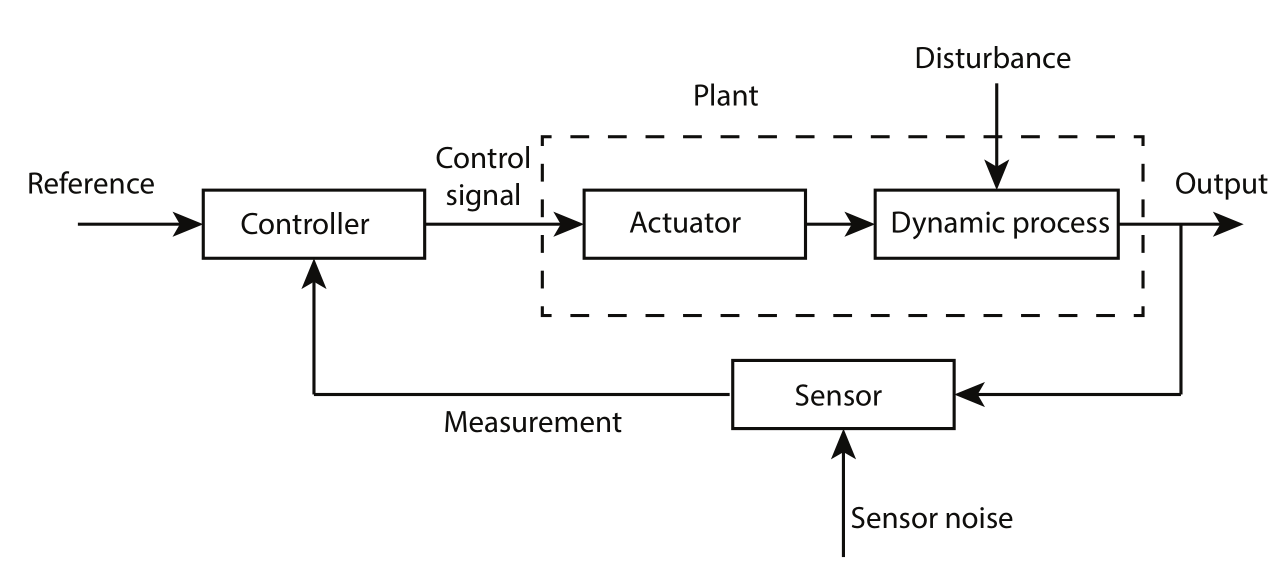
\includegraphics[width=4in]{fig/800px-Feedback_loop_with_descriptions.svg.png}
  \caption{A typical control system}\label{fig_control_loop}
\end{figure}

A closed-loop system uses a measurement of the output signal and a comparison with the desired output to generate an error signal that is used by the controller to adjust the actuator. One of the key concept in the principle of automatic control lies in feedback control.

Despite the cost and increased system complexity, closed-loop feedback control has the following advantages:
\begin{itemize}
  \item Decreased sensitivity of the system to variations in the parameters of the process
  \item Improved rejection of the disturbances.
  \item Improved reduction of the steady-state error of the system.
\end{itemize}

\begin{figure}
  \centering
  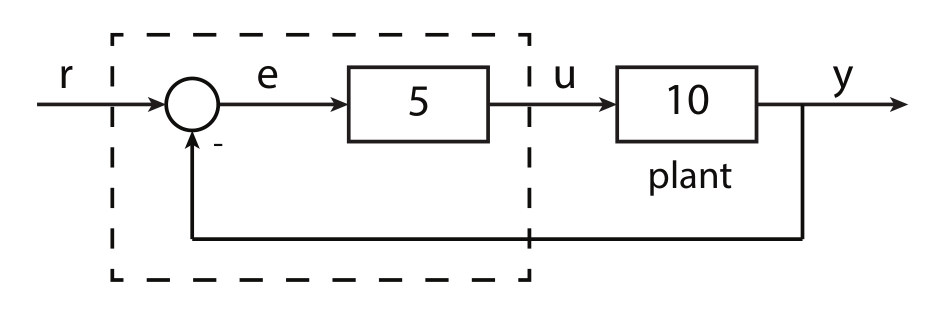
\includegraphics[width=1.8in]{fig/fig_control_example.png}
  \caption{A closed loop control system}\label{fig_control_system}
\end{figure}


\paragraph{Example} A control system is shown as figure \ref{fig_control_system}.

Look at transfer functions from r to y:

\begin{center}
    \begin{tabular}{c|c|c}
      %\hline
      % after \\: \hline or \cline{col1-col2} \cline{col3-col4} ...
        & Open Loop & Closed Loop \\
        \hline
      $\frac{y}{r}$ & $\frac{1}{10} \cdot 10 = 1$ & $\frac{5 \cdot 10}{1+5 \cdot 10} = \frac{50}{51} \approx 0.98$ \\
      %\hline
    \end{tabular}
\end{center}

We want $\frac{y}{r}=1$, so at first glance, it looks like open-loop is better than closed-loop. However, consider what happens if it turns out our plant model was wrong(or changes), so that really G=15. Then

\begin{center}
    \begin{tabular}{c|c|c}
      %\hline
      % after \\: \hline or \cline{col1-col2} \cline{col3-col4} ...
        & Open Loop & Closed Loop \\
        \hline
      $\frac{y}{r}$ & $\frac{1}{10} \cdot 15 = 1.5$ & $\frac{5 \cdot 15}{1+5 \cdot 15} = \frac{75}{76} \approx 0.9868$ \\
      %\hline
    \end{tabular}
\end{center}

That is, if the plant gain changes by 50\%, the transfer function of the open-loop system will vary by -5\%. However, the transfer function of the closed-loop system will vary by only 0.66\% (in this case).

\subparagraph{Big Idea} High gain control loop reduces the sensitivity of
the control system to variations in the plant.

\subsubsection{Time Domain Specifications}
Given a 2nd order system transfer function:
$$H(s)=\frac{\omega ^2 _n}{s^2+2\zeta \omega _n s + \omega ^2 _n} $$

Typical response is shown in figure \ref{fig_step_response}.
\begin{figure}
  \centering
  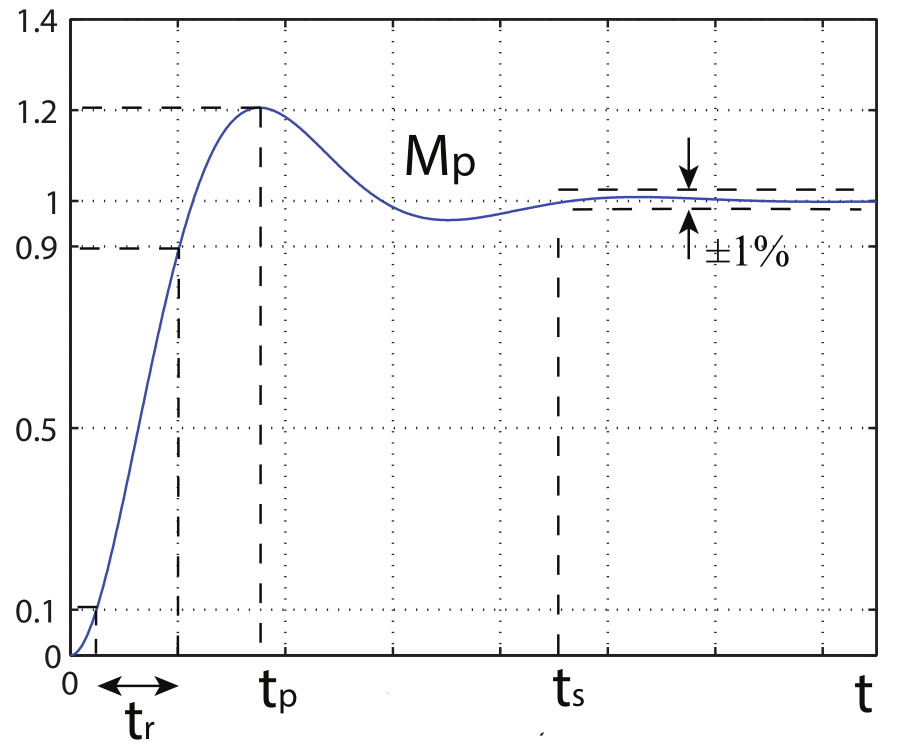
\includegraphics[width=2.5in]{fig/cntr_step.png}
  \caption{step response of a 2nd order system}\label{fig_step_response}
\end{figure}

$M_p$ = peak overshoot

$t_r$ = rise time (10\% to 90\%)

$t_s$ = settling time (1\%)

$t_p$ = time of peak

The step response of H(s) is:
$$h_s(t)=1-e^{-\zeta \omega _n t}(\textrm{cos}(\omega _d t) + \frac{1}{\sqrt{1-\zeta ^2 }}\textrm{sin}(\omega _d t))$$

\subsubsection{Übertragungsfunktion}
Die Übertragungsfunktion oder auch Systemfunktion beschreibt in der ingenieurwissenschaftlichen Systemtheorie mathematisch die Beziehung zwischen dem Ein- und Ausgangssignal eines dynamischen Systems im Frequenzraum.

$$G(s) = \frac{Y(s)}{U(s)} = \frac{\mathcal L \{ y(t) \} }{\mathcal L\{ u(t) \} }$$

%\subsubsection{Second Order System}
%
%$$\Phi(s)= \frac{1}{T^2s^2+2\zeta Ts+1}=\frac{\omega^2_n}{s^2+2\zeta \omega_n s+\omega^2_n}$$
%
%$\omega_n$ is natural frequency, and $\zeta$ is damping ratio.

\subsubsection{Stability}
Stability of closed-loop feedback systems is central to control system design. A stable system should exhibit a bounded output if the corresponding input is bounded (BIBO stable).

\paragraph{The Routh Stability Criterion} The closed-loop system is stable if $$\Re(p_i)<0, \forall i$$

Can we tell if the system is stable, without actually solving for the roots?

For \emph{Routth Array}, if all of its coefficient is positive, then the system$$a_ns^n+a_{n-1}s^{n-1}+\dots+a_1s+a_0=0$$is stable.


\begin{tabular}{ccccc}
  %\hline
  % after \\: \hline or \cline{col1-col2} \cline{col3-col4} ...
  Row n: & $a_n$ & $a_{n-2}$ & $a_{n-4}$ & $\dots$ \\
  Row n-1: & $a_{n-1}$ & $a_{n-3}$ & $a_{n-5}$ & $\dots$ \\
  Row n-2: & $b_1$ & $b_2$ & $b_3$ & $\dots$ \\
  Row n-3: & $c_1$ & $c_2$ & $c_3$ & $\dots$ \\
  $\vdots$ &   & $\ddots$ &   &   \\
  Row 3: & * & * &  &\\
  Row 2: & * &   &   &   \\
  Row 1: & * &   &   &   \\
  %\hline
\end{tabular}

The number of unstable poles is the number of sign changes in the first column of the array.

\paragraph{Wurzelortskurve}

$$G_0(s) = k \hat{G}_0(s) = k \frac{\Pi_{i=1}^{q}(s-s_{0i})}{\Pi_{i=1}^{n}(s-s_i)}$$

\begin{enumerate}
  \item Ursprung/Ende: Jeder Ast der Wurzelortskurve beginnt in einem Pol der offenen Kette $G_0$ und endet in einer Nullstelle der offenen Kette, oder im Unendlichen.
  \item Asymptoten: Für große Verstärkungen nähern sich die Äste Geraden asymptotisch an. Die Anzahl der Asymptoten ist $n-q$. Die Asymptoten haben für $k>0$ Neigungswinkel $\phi_\mathrm{As} = \frac{\pi+ l \cdot 2 \pi}{n-q}, \quad l=0,1,...,n-q-1$ und schneiden sich im gemeinsamen Schnittpunkt (Wurzelschwerpunkt) $s_\mathrm{As} = \frac{\sum_{i=1}^{n}s_i-\sum_{i=1}^{q}s_{0i}}{n-q}$.
  \item Reelle Achse: Zur eigentlichen Wurzelortskurve gehören genau die Punkte $s$ der reellen Achse, für die die Anzahl der von dort aus gesehen rechts gelegenen reellen kritischen Stellen (Nullstellen und Pole) ungerade ist. Alle übrigen Punkte auf der reellen Achse gehören zur komplementären WOK ($k<0$). Jeder Punkt auf der reellen Achse ist also Teil einer WOK: entweder Teil der eigentlichen WOK ($k>0$) oder Teil der komplementären WOK ($k<0$).
  \item Verzweigungs- und Vereinigungspunkte: Verzweigungs- und Vereinigungspunkte sind genau solche Punkte, die sowohl die Phasenbedingung als auch die Gleichung $\sum_{i=1}^{q} \frac{1}{s-s_{0i}} = \sum_{i=1}^{n}\frac{1}{s-s_i}$ erfüllen.
\end{enumerate}


\paragraph{Frequency Criteria} If the gain for frequencies which have phase delay over $-180^\circ$ is greater than 1, then the system has positive feedback loop for those frequencies, which may cause the system unstable.

\subparagraph{Bode-Diagramm} Ein Bode-Diagramm beschreibt den Zusammenhang zwischen einer harmonischen Anregung („schwingung“) an einem Eingang des Systems und dem zugehörigen Ausgangssignal im stationären Zustand, d.h. für t→∞.

\subsubsection{PID controller}
\begin{itemize}
  \item Increase \textbf{P (proportional)} would speed up the system response, but decrease system damping.
  \item Increase \textbf{I (integral)} would reduce system steady-state error, but may cause overshoot.
  \item Increase \textbf{D (derivative)} would increase system damping, but is affected by noise.
\end{itemize}

\subsubsection{Compensation}
Compensation is the use of a dynamic controller $K(s)$ (as opposed to proportional control) to improve the system's stability and error characteristic.

\paragraph{Lead Compensation}

When the phase margin doesn't meet the stability requirement, then Lead Compensation may be deployed to acquire lower phase lag. One problem with PD controller is that the gain gets large at high frequencies. So instead use lead compensator:

$$G_c(s)=\frac{1+\alpha Ts}{1+Ts}, \alpha >1$$

\begin{figure}
  \centering
  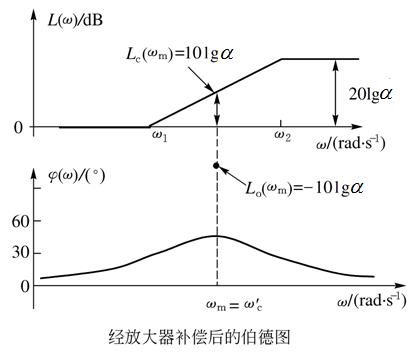
\includegraphics[width=2.4in]{fig/Lead_Compensation.png}
  \caption{Bode Diagram of Lead Compensation}\label{fig_lead}
\end{figure}


\paragraph{Lag Compensation}

In the situation where stable gain is expected to be enlarged, with little influence on dynamic gain, then Lag Compensation is the choice.

$$G_c(s)=\frac{\beta Ts+1}{Ts+1}$$

\begin{figure}
  \centering
  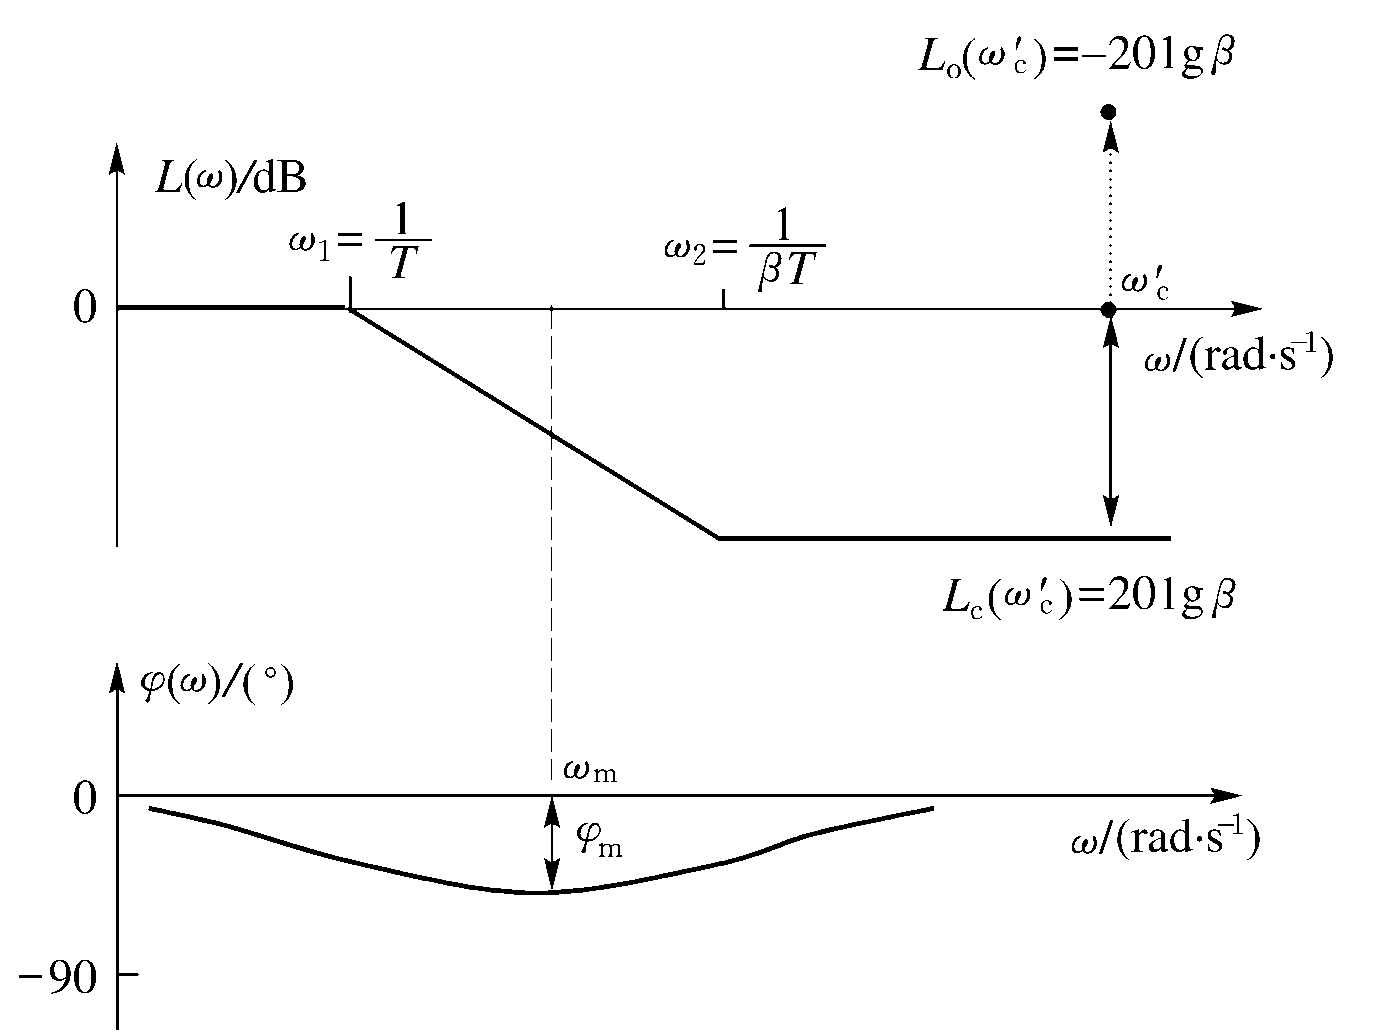
\includegraphics[width=3.5in]{fig/Lag_Compensation.png}
  \caption{Bode Diagram of Lag Compensation}\label{fig_lag}
\end{figure}


%\textbf{We look primarily at four types of compensation:}
%
%$
%\left.
%\begin{aligned}
%  \textrm{PD Control} \\
%  \textrm{Lead Compensation}
%\end{aligned}
%\right\}
%$ used primarily to add lead at the crossover frequency,
% allowing the compensated system to have a faster speed of response and/or have more damping.
%
%$
%\left.
%\begin{aligned}
%  \textrm{PI Control} \\
%  \textrm{Lag Compensation}
%\end{aligned}
%\right\}
%$ used primarily to increase the frequency response magnitude at low frequencies, reducing steady-state tracking errors.

\subsubsection{State Space(Zustandsraumdarstellung)}
The state-space representation (also known as the ``time-domain approach'') provides a convenient and compact way to model and analyze systems with multiple inputs and outputs.

\begin{figure}
  \centering
  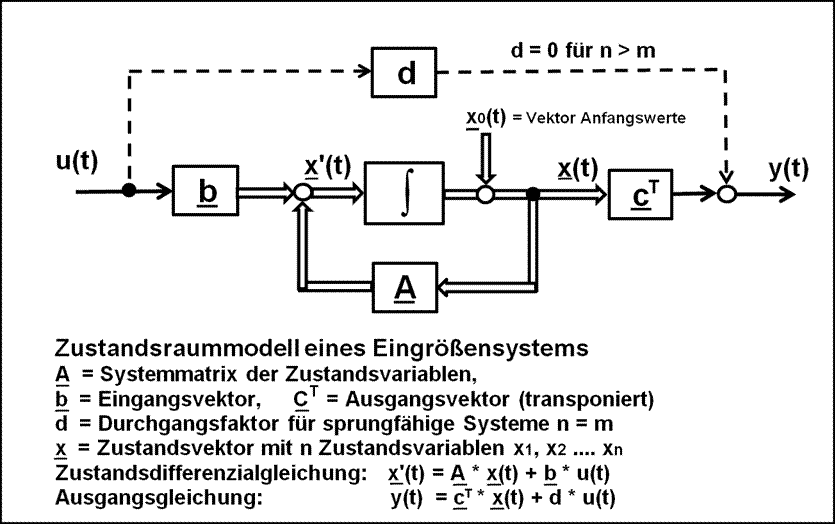
\includegraphics[width=4.5in]{fig/Zustandsraummodell_eines_eingroessensystems.png}
  \caption{Symbolisches Blockschaltbild eines Modells eines Übertragungssystems in der Zustandsraumdarstellung für ein Eingrößensystem.}\label{fig_Zustandraumdarstellung}
\end{figure}

\paragraph{State} The internal state variables are the smallest possible subset of system variables that can represent the entire state of the system at any given time.

\paragraph{Controllability} State controllability condition implies that it is possible – by admissible inputs – to steer the states from any initial value to any final value within some finite time window.  Au\ss erdem, Ausgangssignale des Systems gilt als Steuerbarkeit auch.
%A continuous time-invariant linear state-space model is controllable if and only if
%\begin{equation*}
%  \textrm{rank}
%  \begin{bmatrix}
%    B & AB & A^2B & \dots & A^{n-1}B
%  \end{bmatrix}=n
%\end{equation*}

\paragraph{Observability} Observability is a measure for how well internal states of a system can be inferred by knowledge of its external outputs.
%A continuous time-invariant linear state-space model is observable if and only if
%\begin{equation*}
%  \textrm{rank}
%  \begin{bmatrix}
%    C \\
%    CA \\
%    \vdots \\
%    CA^{n-1}
%  \end{bmatrix}=n
%\end{equation*}

%\includepdfmerge{includes/control_glossar.pdf, 1-12}

\paragraph{Beobachter}

Häufig können aus technischen oder kommerziellen Gründen nicht alle Zustandsvariablen gemessen werden. Deshalb werden einzelne nicht messbare Zustandsvariablen aus den bekannten und vorhandenen Eingangs- und Ausgangsgrößen der Regelstrecke errechnet. Zustandsbeobachter, die diese Aufgabe durchführen, sind zusätzliche Regelsysteme. Sie rekonstruieren Zustandsvariable aus dem Verlauf der Ein- und Ausgangsgrößen an einem Modell der Regelstrecke.

\subsection{Digital Signal Processing(Bilingual)}
This course, to be more specific, talks about how to analyze discrete time signals. I've learnt from this course, how to handle discrete time signal, the FFT Algorithm, how to design a digital filter(IIR and FIR).

\subsubsection{Objekt: Was ist ein Signal?}

Ein digitales Signal ist, im Gegensatz zu den kontinuierlichen Funktionen der analogen Signalverarbeitung, diskret in Zeit- und Wertebereich, also eine Folge von Elementarsignalen (z. B. Rechteckimpulsen). Diese Folge entsteht meist in einem zeit- oder ortsperiodischen Messprozess. So wird zum Beispiel Schall über die Auslenkung einer Membran oder Verbiegung eines Piezokristalls in eine elektrische Spannung umgewandelt und diese Spannung mittels eines AD-Wandlers zeitperiodisch wiederholt in digitale Daten konvertiert. Solch ein realistischer Messprozess ist endlich, die entstehende Folge besitzt einen Anfangsindex $\alpha$ und einen Endindex $\omega$.

\begin{figure}
  \centering
  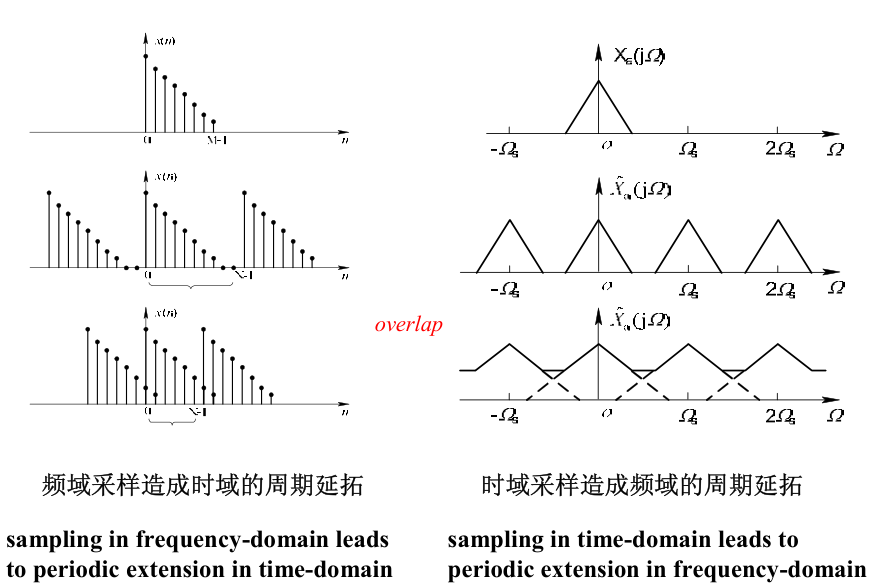
\includegraphics[width=4.2in]{fig/dsp_relationship.png}
  \caption{Relationship between time domain and frequency domain sampling}\label{fig_dsp_sampling}
\end{figure}

\subsubsection{DFT}
A periodic sequence $\tilde{x}(n)=\tilde{x}(n+rN), r\in Z$ can be represented by a Fourier series $\tilde{x}(n)=\displaystyle{\sum_{k=0}^{N-1}a_ke^{j\frac{2\pi}{N}kn}}$, where
$$a_k = \frac{1}{N}\displaystyle{\sum_{n=0}^{N-1}\tilde{x}(n)e^{-j\frac{2\pi}{N}kn}}$$

and thus
$$\tilde{X}(k)=Na_k=DFS[\tilde{x}(n)]=\displaystyle{\sum_{n=0}^{N-1}\tilde{x}(n)e^{-j\frac{2\pi}{N}kn}}$$
$$\tilde{x}(n)=IDFS[\tilde{X}(k)]=\frac{1}{N}\displaystyle{\sum_{k=0}^{N-1}\tilde{X}(k)e^{j\frac{2\pi}{N}kn}}$$

Relationship between time domain and frequency domain:
\begin{itemize}
  \item continuous $\leftrightarrow$ nonperiodic
  \item discrete $\leftrightarrow$ periodic
\end{itemize}

\subsubsection{DIT-FFT}
It re-expresses the DFT of an arbitrary composite size $N = N_1N_2$ in terms of smaller DFTs of sizes $N_1$ and $N_2$, recursively, to reduce the computation time to $O(N log N)$.

Separate x(n) into two (N/2)-point sequences consisting of the even-numbered points and odd-numbered points.
$$
\left\{
    \begin{aligned}
      x_1(r) &= x(2r) \\
      x_2(r) &= x(2r+1)
    \end{aligned}
\right.
$$

And then perform Butterfly Computation

$$
\left\{
    \begin{aligned}
      X(k) &= X_1(k)+W_n^kX_2(k) \\
      X(k+\frac{N}{2}) &= X_1(k)-W_n^kX_2(k)
    \end{aligned}
\right.
$$

\begin{figure}
  \centering
  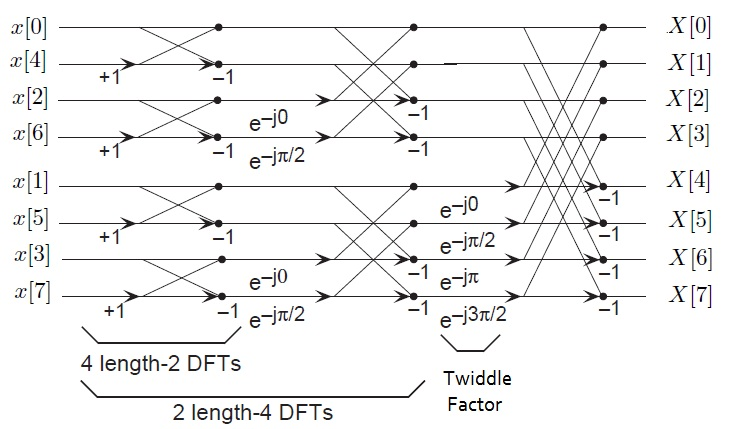
\includegraphics[width=3.5in]{fig/FFt.jpg}
  \caption{Data flow diagram for N=8}\label{fig_fft}
\end{figure}

\subsubsection{IIR Filter}

An IIR Filter of order N the transfer function:

\begin{align*}
H(z) & = \frac{\sum_{i=0}^P b_{i} z^{-i}}{1+\sum_{j=1}^Q a_{j} z^{-j}}
\end{align*}

IIR filters have much better frequency response than FIR filters of the same order. Unlike FIR filters, their phase characteristic is not linear which can cause a problem to the systems which need phase linearity.

\paragraph{Design Flow}

Die Aufgabe des Filterentwurfs ist es, eine rationale Funktion von $z^{-1}$ zu finden, die das Toleranzschema auf dem Einheiskreis $z=e^{j\Omega}$ erf\"ullt.

\begin{figure}
  \centering
  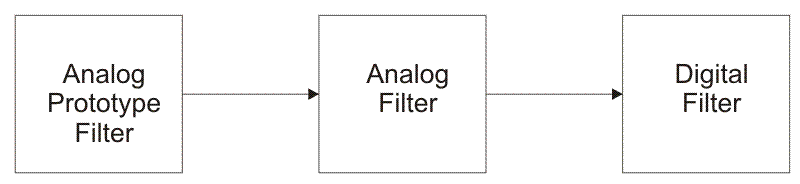
\includegraphics[width=2.5in]{fig/fig3-1-2.png}
  \caption{Block diagram of design method using reference analog prototype filter}\label{fig_iir}
\end{figure}

First step is design analog low-pass filter, whose parameter is selected base on the desired characteristic of IIR filter. The second step is to convert the low-pass one to the desired pass band.

The last step is perform either Transformation via Impulse Invariance ($z_i=e^{s_iT}$, $\omega = \Omega T$), or Bilinear Transformation ($s=\frac{2}{T}\frac{1-z^{-1}}{1+z^{-1}}$, $\Omega = \frac{2}{T}\textrm{tan}(\frac{\omega}{2})$), to convert the filter from analog to digital.

While filter with Transformation via Impulse Invariance has better approximation to the analog filter, bilinear transformation features for its anti-aliasing.

\subsubsection{FIR Filter}
In such cases when it is necessary to have a linear phase characteristic, FIR filters are the only option available. The ideal filter frequency response is used when designing FIR filters using window functions. The objective is to \emph{compute the ideal filter samples}.

FIR filters have finite impulse response, which means the ideal filter frequency sampling must be performed in a finite number of points.

For a FIR filter of order N to have linear phase characteristic, it must have $h[n]=h[N-n]$ or $h[n]=-h[N-n]$.

\paragraph{Design Flow} The FIR filter deseign process can be split into three steps:
\begin{enumerate}
  \item Specifying a window function according to the filter specifications;
  \item Computing the filter order (N) required for a given set of specifications;
  \item Computing FIR filter coefficients according to the obtained window function and ideal filter coefficients;
\end{enumerate}

\begin{figure}
  \centering
  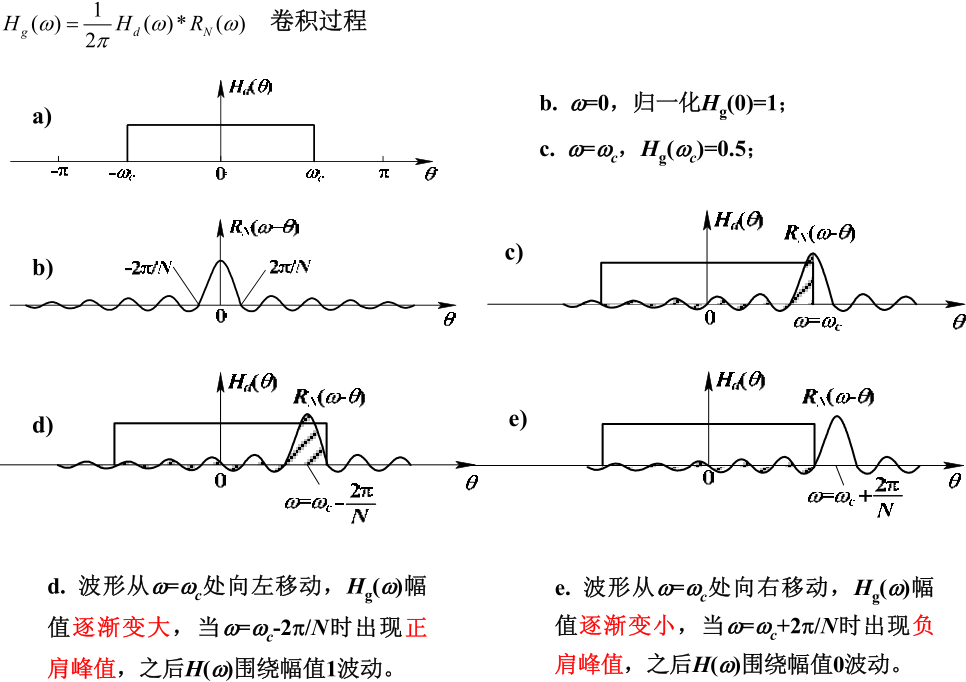
\includegraphics[width=4.5in]{fig/fig_FIR_design.png}
  \caption{FIR design process}\label{fig_FIR_design}
\end{figure}

\section{Physik}
\subsection{College Physics II}
\subsection{College Physics Experiment I}

\subsubsection{Wheatstone bridge}

\begin{figure}
  \centering
  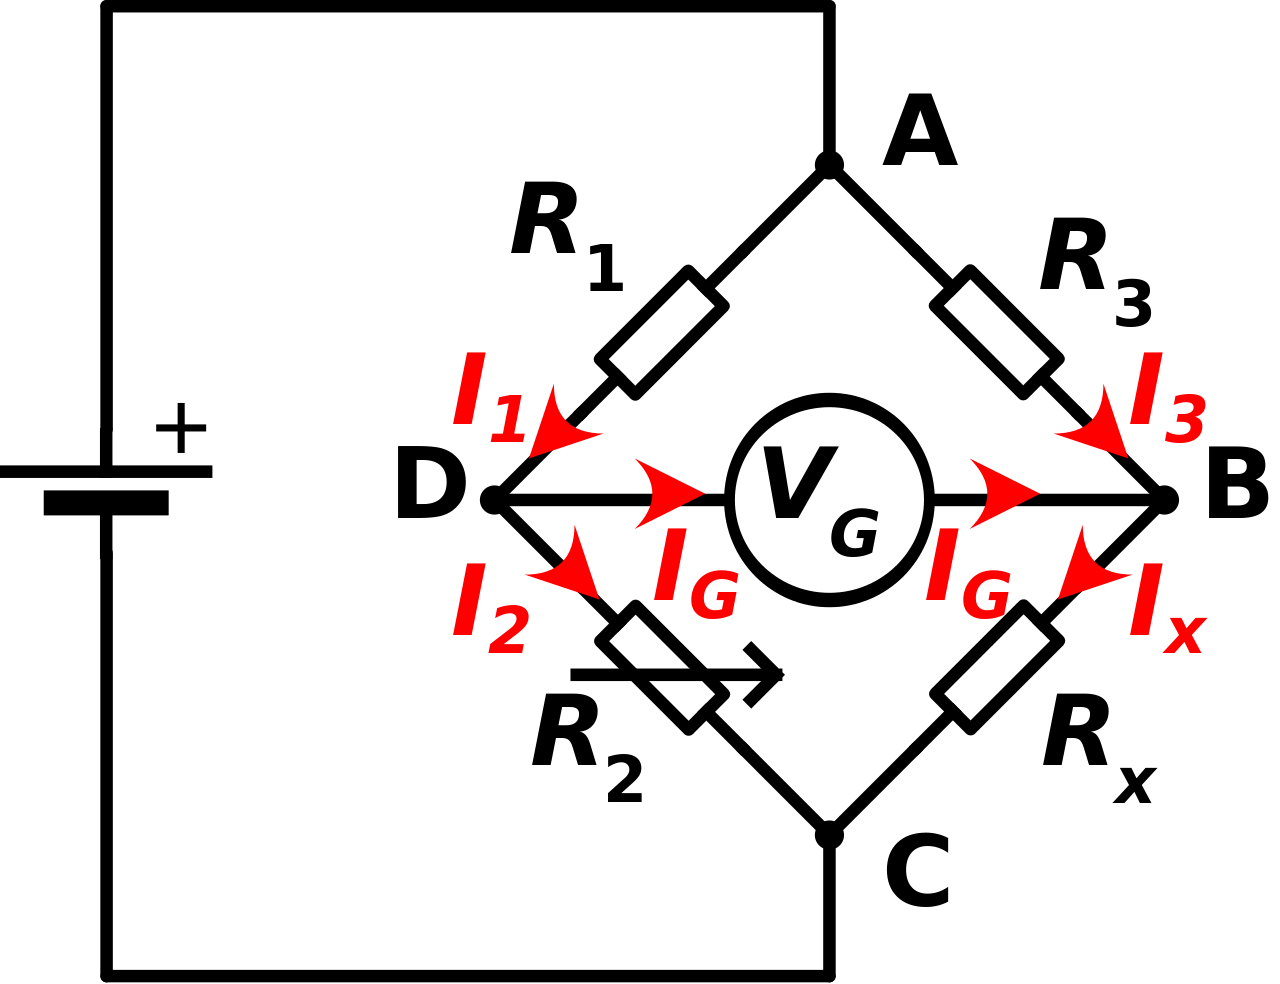
\includegraphics[width=2.5in]{fig/1280px-Wheatstonebridge_current.svg.png}
  \caption{Wheatstone bridge}\label{fig_wheatstonebridge}
\end{figure}

A Wheatstone bridge is an electrical circuit used to measure an unknown electrical resistance by balancing two legs of a bridge circuit, one leg of which includes the unknown component. The primary benefit of a wheatstone bridge is its ability to provide extremely accurate measurements.

From Kirchhoff's Current Law:

\begin{multline*}
  I_3-I_x+I_G=0 \\
  I_1-I_2-I_G=0
\end{multline*}

And from Kirchhoff's Voltage Law:

\begin{multline*}
  (I_3\dot R_3)-(I_G\dot R_G)-(I_1\dot R_1)=0 \\
  (I_x\dot R_x)-(I_2\dot R_2)+(I_G\dot R_G)=0
\end{multline*}

when the bridge is balanced, then $I_G=0$, then

$$
R_x=\frac{R_2\dot I_2\dot I_3\dot R_3}{R_1\dot I_1\dot I_x}
$$

and thus:

$$R_x=\frac{R_3 \dot R_2}{R_1}$$

\subsubsection{Thermocouple}

\paragraph{Seebeck effect} When two dissimilar metals are joined at one end, an electrical potential
called the ``Seebeck voltage'' is generated, which changes proportionally to changes in the temperature at the joint.

\subsection{Basis of Microwave Technique}
The first part of the course reviews the fundamental of electromagnetic, the Maxwell's Equation. Then focus on the basis of microwave technique, which is about Transmission Line, Waveguide, and lastly S-parameters.
\subsubsection{Maxwell's Equation}

All electromagnetic behaviors can ultimately be explained by Maxwell’s four basic equations:
\begin{align*}
  \mbox{Gauss's law   } \nabla \cdot \mathbf{E} &= \frac{\rho}{\varepsilon_0} \\
  \mbox{Gauss's law for magnetism   } \nabla \cdot \mathbf{B} &= 0 \\
  \mbox{Faraday's law of inducton   } \nabla \times \mathbf{E} &= - \frac{\partial \mathbf{B}}{\partial t} \\
  \mbox{Apm\`ere's cicuital law   } \nabla \times \mathbf{B} &= \mu(\mathbf{J}+\varepsilon\frac{\partial \mathbf{E}}{\partial t})
\end{align*}
\subsubsection{Transmission Line}
A transmission line is a specialized cable designed to carry alternating current of radio frequency.
Types of transmission line include parallel line (ladder line, twisted pair), coaxial cable, stripline, and microstrip. Transmission lines become necessary when the length of the cable is longer than a significant fraction of the transmitted frequency's wavelength.

\paragraph{Telegrapher's equations} The telegrapher's equations are a pair of linear differential equations which describe the voltage and current on an electrical transmission line with distance and time
\begin{align*}
  \frac{\partial V(x)}{\partial x} &= -(R+j\omega L)I(x) \\
  \frac{\partial I(x)}{\partial x} &= -(G+j\omega C)V(x)
\end{align*}

Steady-state Telegrapher's equations are:

\begin{align*}
  \frac{\partial ^2 V(x)}{\partial x^2} &= \gamma ^2 LC \cdot V(x) \\
  \frac{\partial ^2 I(x)}{\partial x^2} &= \gamma ^2 LC \cdot I(x)
\end{align*}

where propagation constant $\gamma = \sqrt{(R+j\omega L)(G+j\omega C)} = \alpha + j \beta$.

The real part of the propagation constant is the \emph{attenuation constant}. It causes a signal amplitude to decrease along a transmission line. The \emph{phase constant} is denoted by $\beta = 2\pi / \lambda$. It determines the sinusoidal amplitude/phase of the signal along a transmission line, at a constant time.

\subparagraph{Phase constant versus wavenumber} Phase constant and wavenumber are often treated as the same thing. Indeed, for TEM transmission lines (coax and stripline), the phase constant and wavenumber are equal. Wavequide is one case where you need to understand the difference between the two.

\emph{Wavenumber} is denoted by lower case ``k'', and is a measure of how many cycles a wave has in a given length, for a traveling wave that is frozen in time.

\paragraph{Characteristic impedance}
$$Z_0=\frac{U^+(z)}{I^+(z)}=\sqrt{\frac{R+j\omega L}{G+j\omega C}}$$
The characteristic impedance of a transmission line is the \emph{ratio} of the voltage and current of a wave travelling along the line. When the wave reaches the end of the line, in general, there will be a \textbf{reflected wave} which travels back along the line in the opposite direction.

When this wave reaches the source, it adds to the transmitted wave and the ratio of the voltage and current at the input to the line will no longer be the characteristic impedance. This new ratio is called the \textbf{input impedance}.

$$Z_{in}(z')=\frac{U(z')}{I(z')}=Z_0\frac{Z_l+jZ_0\tan\beta z'}{Z_0+jZ_l\tan\beta z'}$$

\paragraph{Impedance Matching}

If impedance matches, no reflection will be produced along the line, and thus input impedance equals to characteristic impedance.

Impedance matching has the following advantages:
\begin{itemize}
  \item load accepts maximum power output from matched source
  \item power losses is minimum in the matched transmission line
  \item the matched transmission line has the largest power capacity
  \item signal source operates in stable condition
\end{itemize}

\subparagraph{VSWR(Voltage Standing Wave Ratio)}
$$\textrm{reflection coefficient }\Gamma = \frac{V_r}{V_f}=\frac{Z_{in}(z')-Z_0}{Z_{in}(z')+Z_0}$$
Standing Wave Ratio (SWR) is a measure of impedance matching of loads to the characteristic impedance of a transmission line or waveguide.

$$VSWR=\frac{|V_{max}|}{|V_{min}|}=\frac{1+|\Gamma|}{1-|\Gamma|}$$

\begin{figure}
  \centering
  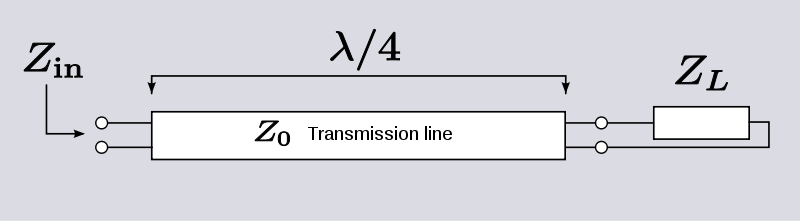
\includegraphics[width=4.2in]{fig/800px-Quarter_wave_impedance_transformer.svg.png}
  \caption{Diagram illustrating how a quarter wavelength transmission line can be used to transform an impedance into its dual.}\label{fig_quarter_wave}
\end{figure}

\subparagraph{QWT (Quarter-wave impedance transformer)} For a $\lambda /4$-length TL, the input impedance is $Z_{in}=Z_1^2 / Z_L$. Adjust $Z_1$ so that $Z_{in}=Z_0$, and find $Z_1=\sqrt{Z_0Z_L}$. By using a quarter-wavelength of transmission line, the impedance of the load ($Z_L$) can be transformed via the above equation.

In general, impedance matching is very important in RF/microwave circuit design. It is relatively simple at a single frequency, but becomes very difficult if wideband impedance matching is desired.

\subparagraph{Smith Chart} Smith chart is a graphical aid or nomogram designed for electrical and electronics engineers specializing in radio frequency (RF) engineering to assist in solving problems with transmission lines and matching circuits.

\begin{figure}
  \centering
  
\includegraphics[width=4.5in]{fig/1300px-Smith_chart_gen.svg.png}
  \caption{Impedance Smith Chart}\label{fig_smith_chart}
\end{figure}

\subsubsection{Waveguide}
Waves propagate in all directions in open space. A waveguide confines the wave to propagate in one dimension, so that, under ideal conditions, the wave loses no power while propagating.

\paragraph{Transverse Mode}

\begin{itemize}
  \item Transverse Electric and Magnetic (TEM),
  \item Transverse Electric (TE) $E_z = 0$ and $H_z \neq 0$
  \item Transverse Magnetic (TM) $E_z \neq 0$ and $H_z = 0$
\end{itemize}

Assume that the waveguide is invariant in the z-direction, and that the wave is propagating in z as $e^{-j\beta z}$. From $\nabla \times \bar{E}=-j\omega \mu \bar{H}$, we find
$$H_x=\frac{j}{k_c^2}(\omega \varepsilon \frac{\partial E_z}{\partial y}-\beta \frac{\partial H_z}{\partial x})$$
where $k_c^2\equiv k^2-\beta ^2$ and $k^2=\omega ^2 \mu \varepsilon$.

Most important point: all transverse components of $\bar{E}$ and $\bar{H}$ can be determined from only the axial components $E_z$ and $H_z$.

\paragraph{Dominant Mode} The mode with the lowest cutoff frequency is termed the dominant mode of the guide. In rectangular and circular (hollow pipe) waveguides, the dominant modes are designated the $TE_{1,0}$ mode. Single mode operation is most often the preferred application for hollow waveguides.

$$\lambda_c=\frac{2}{\sqrt{(\frac{m}{a})^2+(\frac{n}{b})^2}}$$

\subsubsection{S-parameters}

%The scattering matrix is a mathematical construct that quantifies how RF energy propagates through a multi-port network. The S-matrix is what allows us to accurately describe the properties of incredibly complicated networks as simple ``black boxes''. For an RF signal incident on one port, some fraction of the signal bounces back out of that port, some of it scatters and exits other ports (and is perhaps even amplified), and some of it disappears as heat or even electromagnetic radiation.

\begin{figure}
  \centering
  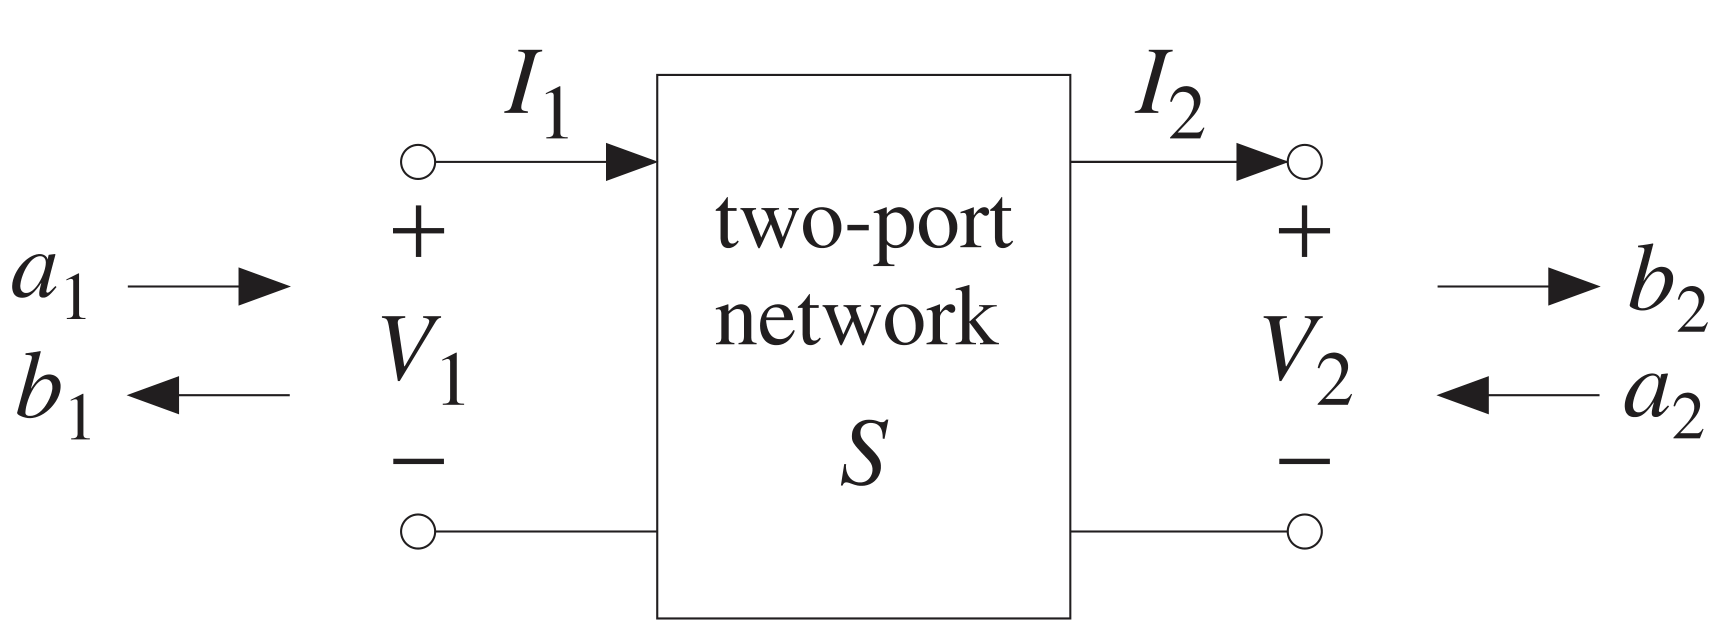
\includegraphics[width=3.2in]{fig/S_parameter.png}
  \caption{Two-port network}\label{fig_s_parameter}
\end{figure}

%\begin{align*}
%  S_{11} &= \frac{b1}{a1} \\
%  S_{12} &= \frac{b1}{a2} \\
%  S_{21} &= \frac{b2}{a1} \\
%  S_{22} &= \frac{b2}{a2}
%\end{align*}

Linear networks, or nonlinear networks operating with signals sufficiently small to cause the networks to respond in a linear manner, can be completely characterized by parameters measured at the network terminals (ports) without regard to the contents of the networks.

S-parameters are important in microwave design because they are easier to measure and work with at high frequencies than other kinds of parameters.

\[
\begin{bmatrix}
   b_1 \\
   b_2
\end{bmatrix}
=
\begin{bmatrix}
   S_{11} & S_{12} \\
   S_{21} & S_{22}
\end{bmatrix}
\begin{bmatrix}
   a_1 \\
   a_2
\end{bmatrix}
\]

The parameters $S_{11}$, $S_{22}$ have the meaning of reflection coefficients, and $S_{12}$, $S_{21}$, have the meaning of transmission coefficients.

S-parameters change with the measurement frequency, so frequency must be specified for any S-parameter measurements stated, in addition to the characteristic impedance or system impedance.

\subsection{Engineering Optics}
In this course, I've learnt the general principles of Geometric Optics, Apertures and Stops, Aberrations, and the structure of Optical Instruments.

\subsubsection{General Principles}

\paragraph{Rectilinear Propagation}
\begin{itemize}
  \item left alone, rays don't change direction
  \item rays change direction when they encounter a new medium according to Snell's Law
\end{itemize}

\paragraph{Snell's Law} When a ray of light strikes a new medium, it may be reflected or it may traverse the boundary with a change of direction(refraction).

\subparagraph{Refractive Index} The \emph{refractive index} describes how light propagates through a medium. It is defined as:

$$n=\frac{c}{v}$$

where $c$ is the speed of light, and $v$ is the phase velocity of light in the medium.

\begin{figure}
  \centering
  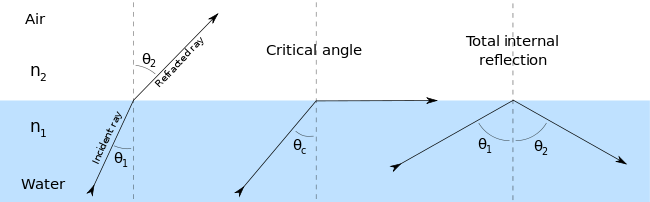
\includegraphics[width=4.5in]{fig/650px-RefractionReflextion.svg.png}
  \caption{Refraction of light at the interface between two media.}\label{fig_snell}
\end{figure}

$$n_1\textrm{sin}\theta _1 = n_2 \textrm{sin}\theta _2$$

\subparagraph{Total internal reflection} When a ray strikes a medium boundary at a larger angle than critical angle, then the ray cannot pass through and is entirely reflected.

%\paragraph{Stigmatic Condition (perfect imaging)} If a system is perfectly stigmatic for A and A', then $L(AA')=constant$.
%
%\paragraph{Refraction of a Light Ray at a Single Surface}
%
%\begin{equation*}
%\left\{
%  \begin{aligned}
%    \textrm{sin}I =& (L-r)\frac{\textrm{sin}U}{r} \\
%    \textrm{sin}I' =& \frac{n}{n'}\textrm{sin}I \\
%    U' =& U+I-I'\\
%    \frac{\textrm{sin}I'}{L'-r}=& \frac{\textrm{sin}U'}{r}
%  \end{aligned}
%\right.
%\end{equation*}
%$$\Rightarrow L'= r(1+\frac{\textrm{sin}I'}{\textrm{sin}U'})$$
%\begin{align*}
%  \mbox{laberal magnification:   } \beta &= m = \frac{y'}{y} \\
%  \mbox{longitudinal magnification:   } \alpha &=m_L= \frac{dz'}{dz} \\
%  \mbox{Helmholz invariant:   } L &=nyu=n'y'u'(paraxial marginal)
%\end{align*}
%
%\paragraph{Rays close to the optic axis:}
%$$\frac{1}{s}+\frac{1}{s'}= \frac{2}{R}$$
%
%where s is the object distance to the Kugel on the axis.

\begin{figure}
  \centering
  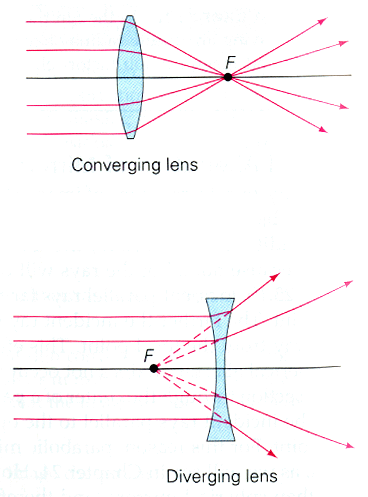
\includegraphics[width=2.7in]{fig/lenses.png}
  \caption{lens imaging}\label{fig_lens_imaging}
\end{figure}

\subsubsection{Graphical Method - Principal Ray Tracing}
\begin{itemize}
  \item an incident ray pass the 2nd focus point parallel to the optic axis.
  \item a ray through centre of lens doesn't deviate.
  \item a ray through 1st focus point refract parallel to the optical axis.
\end{itemize}

\paragraph{Principal Planes} Conjugate planes for which transverse magnification is unity ($\beta=1
$) , its intersection with axis are named \emph{principal points}.

\begin{figure}
  \centering
  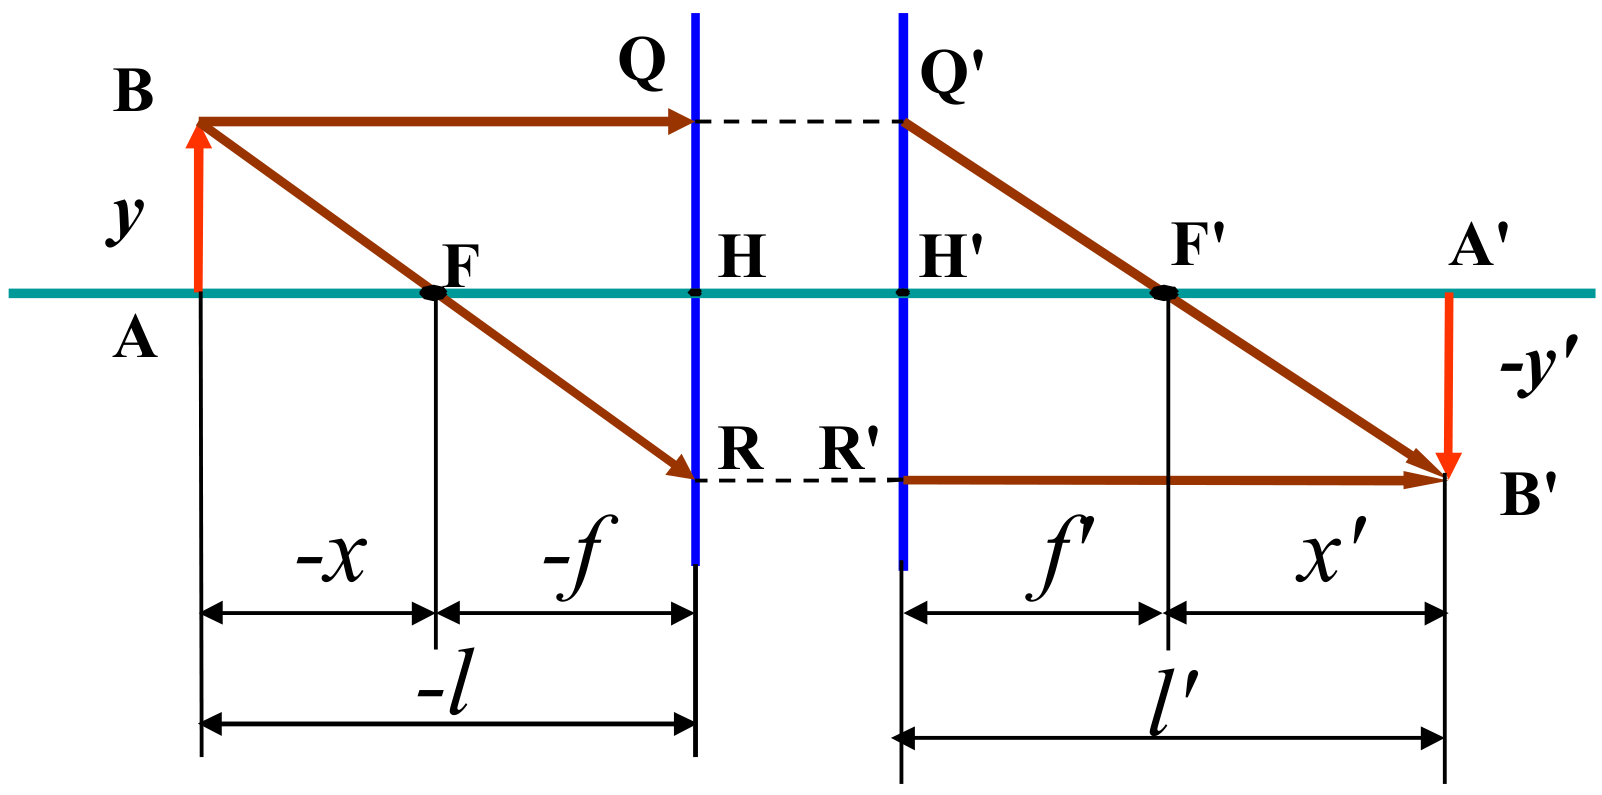
\includegraphics[width=3.2in]{fig/newtons_equation.png}
  \caption{Optical System}\label{fig_newtons_equation}
\end{figure}

\paragraph{Newton's Equation}

$$xx' =ff'$$ or $$\frac{x'}{l'}+\frac{x}{l} = 1$$

\paragraph{Gauss's Equation}

$$\frac{f'}{l'}+\frac{f}{l}=1$$

\subsubsection{Apertures and stops}

\paragraph{Chief Ray} Starts from off-axis object, goes through the cnetre of the Aperture, and marginal ray goes through the edge of the aperture.

\paragraph{Aperture}

The aperture and focal length of an optical system determine the cone angle of a bundle of rays that come to a focus in the image plane.

\begin{itemize}
  \item largest possible \emph{angle} for object of zero height
  \item depends on where the object is located
  \item determines the system resolution, light transmission efficiency, and the depth of field
\end{itemize}

NA: numerical aperture

$$NA=n\textrm{sin}\alpha $$

which is a property of cones of light.

\subparagraph{Aperture Stop} The physical element which limits the nagle of acceptance of the imaging system. The image of the \emph{aperture stop} in \emph{object} (image) space

\begin{figure}
  \centering
  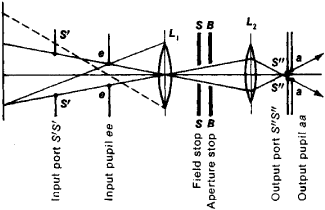
\includegraphics[width=3.0in]{fig/gsed_0001_0015_0_img3897.png}
  \caption{Aperture and stops}\label{fig_Aperture_and_stops}
\end{figure}

\subparagraph{Field Stop} The element that limits the size or angular breadth of an object that can be imaged by the system is called the field stop. For cameras, the size of the film or CCD detector determines the maximum image size and serves as the field stop. The images of the field stop is called \emph{window}. Filed stop alse defines the Field of View(FoV).

\paragraph{Depth of Field} Depth of Field is the distance between the nearest and farthest objects in a scene that appear acceptably sharp in an image.

%\begin{equation*}
%\left\{
%  \begin{aligned}
%    \delta z &=\frac{p}{NA}\\
%    \Delta &=\frac{\delta z}{\alpha}
%  \end{aligned}
%\right.
%\end{equation*}

\subsubsection{Aberrations}
\paragraph{Geometrical Aberrations}
\begin{itemize}
\item spherical aberration
\item astigmatism
\item coma
\item curvature of field
\item distortion
\end{itemize}

\begin{figure}
  \centering
  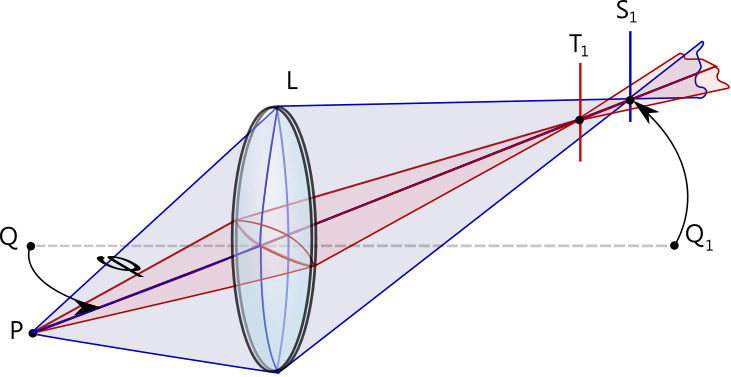
\includegraphics[width=3.0in]{fig/731px-Astigmatism.svg.png}
  \caption{astigmatism}\label{fig_astigmatism}
\end{figure}

\begin{figure}
  \centering
  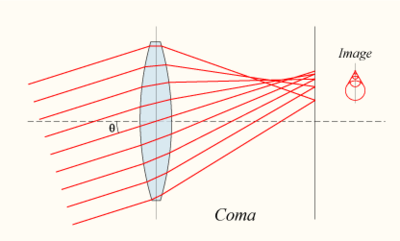
\includegraphics[width=3.0in]{fig/400px-Lens-coma.png}
  \caption{coma}\label{fig_coma}
\end{figure}

\begin{figure}
  \centering
  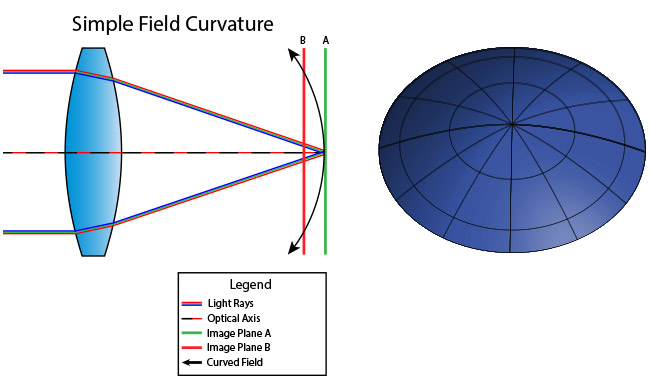
\includegraphics[width=3.0in]{fig/curvature_of_field.png}
  \caption{curvature of field}\label{fig_curvature_of_field}
\end{figure}

\begin{figure}
  \centering
  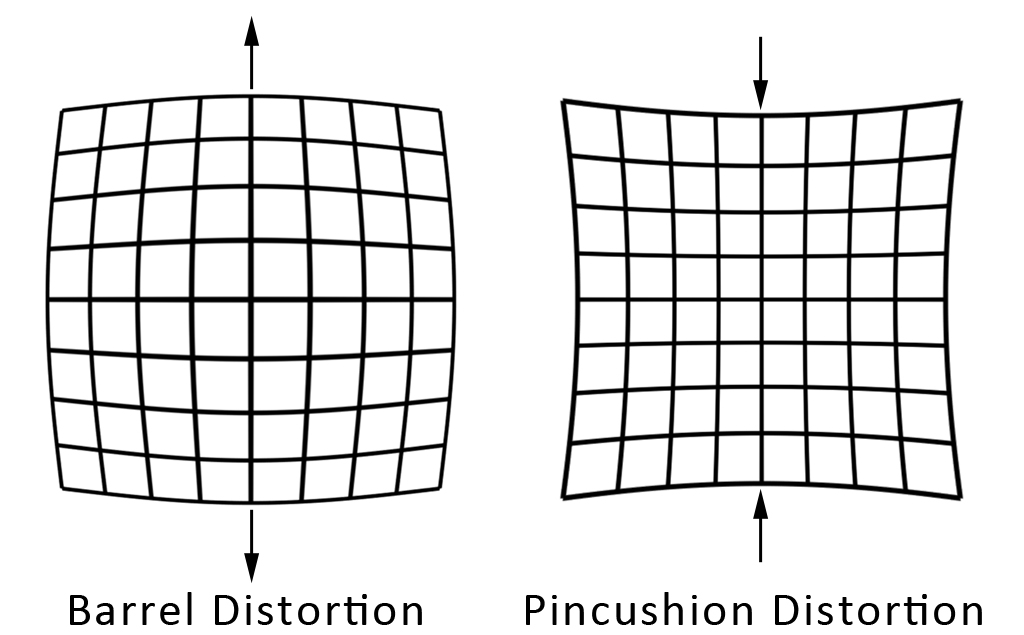
\includegraphics[width=3.0in]{fig/distortion.png}
  \caption{distortion}\label{fig_distortion}
\end{figure}

\subsubsection{Optical Instruments}

\begin{figure}
  \centering
  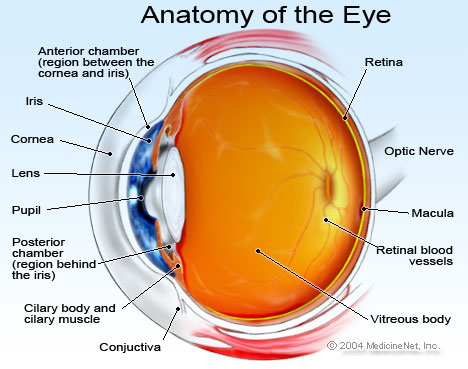
\includegraphics[width=3.0in]{fig/eye.png}
  \caption{eye}\label{fig_eye}
\end{figure}

\paragraph{Near Point} Most people cannot focus on an object that is closer than a certain distance known as the \emph{near point} ($D = 25cm$).

\begin{figure}
  \centering
  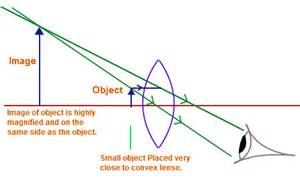
\includegraphics[width=3.0in]{fig/magnifying_glass.png}
  \caption{Magnifying Glass}\label{fig_magnifying_glass}
\end{figure}

\begin{figure}
  \centering
  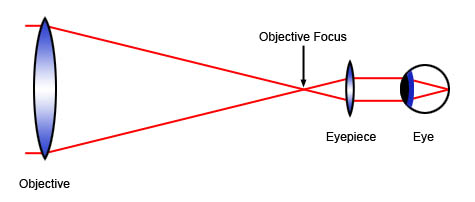
\includegraphics[width=3.0in]{fig/telescope.png}
  \caption{Telescope}\label{fig_telescope}
\end{figure}

\begin{figure}
  \centering
  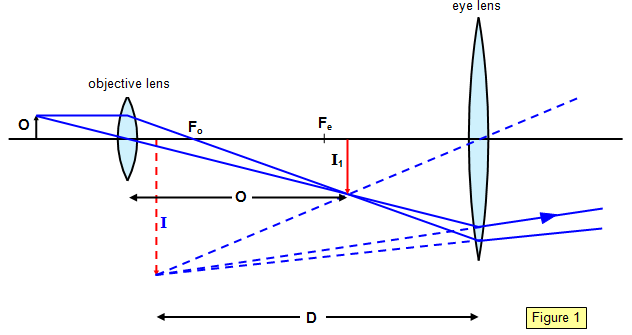
\includegraphics[width=3.0in]{fig/microscope.png}
  \caption{Microscope}\label{fig_microscope}
\end{figure}
\section{Elektrotechnik}
\subsection{Electric Circuit III}

\subsubsection{Passive Sign Convention}
The convention defines electric power flowing out of the circuit into an electrical component as positive, and power flowing into the circuit out of a component as negative.

\subsubsection{Nodal analysis}

\subsubsection{Mesh analysis}

\subsubsection{Thévenin's theorem}

Any linear electrical network with voltage and current sources and only resistances can be replaced at terminals A-B by an equivalent voltage source $V_{th}$ in series connection with an equivalent resistance $R_{th}$.

\subsubsection{Norton's theorem}

Any linear electrical network with voltage and current sources and only resistances can be replaced at terminals A-B by an equivalent current source $I_{NO}$ in parallel connection with an equivalent resistance $R_{NO}$.

\subsubsection{Line Voltage/Phase Voltage}

Line voltage is the voltage measured between any two lines in a three-phase circuit. Phase voltage is the voltage measured across a single component in a three-phase source or load.

For ``Y'' circuits:
\begin{align*}
  E_{line}&=\sqrt{3}E_{phase} \\
  I_{line}&=I_{phase}
\end{align*}

For $\Delta$ circuits:

\begin{align*}
  E_{line}&=E_{phase} \\
  I_{line}&=\sqrt{3}I_{phase}
\end{align*}

\subsection{Introduction to Analog Electronic Technology I}

In this course we learned semiconductor diodes and Bipolar Junction Transistor, and basic amplifying circuits. We also learned the operational amplifying circuits and the feedback.

\paragraph{PN Junction} PN junctions are elementary "building blocks" of most semiconductor electronic devices such as diodes, transistors. A PN junction is a boundary or interface between p-type and N-type.

After joining p-type and n-type semiconductors, electrons from the n region near the PN interface tend to diffuse into the p region. As electrons diffuse, they leave positively charged ions (donors) in the n region. Likewise, holes from the p-type region near the p–n interface begin to diffuse into the n-type region, leaving fixed ions (acceptors) with negative charge. The regions nearby the p–n interfaces lose their neutrality and become charged, forming the space charge region or depletion layer. Its resistance is very big.

\paragraph{Transistor} A bipolar junction transistor (BJT or bipolar transistor) is a type of transistor that relies on the contact of two types of semiconductor for its operation.
BJTs come in two types, or polarities, known as PNP and NPN. The regions of a BJT are called emitter, collector, and base.

\paragraph{Filter} Passive filters are based on combinations of resistors (R), inductors (L) and capacitors (C). Because they do not depend on an external power supply and/or they do not contain active components such as transistors.

\subsection{Analog Electronics Experiments}

\newpage 
\subsection{Fundamental Technology of Digital Electronics I}

\newpage

\subsection{Curriculum Design of Electronics II}

The student grouped to design a digital frequency meter. The structure is shown in figure \ref{fig_digit_meter}.

\begin{figure}
  \centering
  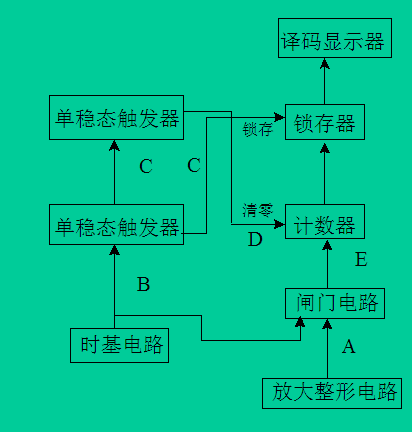
\includegraphics[width=2.3in]{fig/curriculum_circuit_design.png}
  \caption{Digital Frequency Meter}\label{fig_digit_meter}
\end{figure}

\subsection{High Frequency Electronic Circuit}
High Frequency ranges from \SIrange{0.3}{300}{\mega\hertz}. I learnt from this course the general structure of a radio communication system, it is composed of transmitter and receiver. The course mainly focus on the following:
\begin{enumerate}
  \item Signal Amplifying

  small-signal RF amplifier, RF power amplifier

  \item Signal Generation

  oscillator

  \item Signal Modulation

  frequency modulation, phase modulation

  \item Feedback Control

  phase lock loop
\end{enumerate}
\subsubsection{Signal Amplifying}

\paragraph{Resonant Circuit} Resonant circuit eliminate the unwanted frequencies due to the nonlinearty of components. The loaded Q-factor is a measure of the selectivity of a resonant circuit:

$$Q=\frac{f_{center}}{\Delta f}=\frac{R_p}{X_p}$$

\begin{figure}
  \centering
  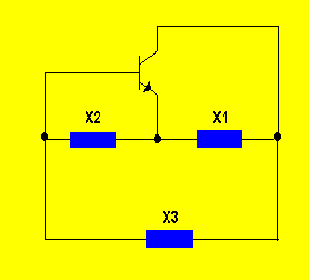
\includegraphics[width=1.5in]{fig/fig_LC_resonant.png}
  \caption{LC Resonant Circuit, $|X_3|=|X_1+X_2|$ and $X_1+X_2+X_3=0$.}\label{fig_lc_resonant}
\end{figure}

\paragraph{Small-Signal RF Amplifier} We can module a small-signal RF transistor as a two-port network with Y-parameters, as shown in firugre \ref{fig_rf_signal_amp}. The input port of transistor is transformer's secondary winding.

\begin{figure}
  \centering
  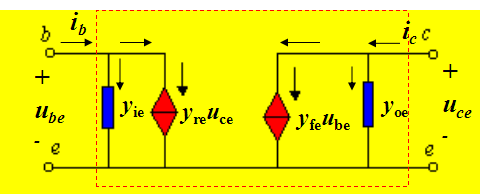
\includegraphics[width=2.5in]{fig/fig_rf_signal_amp.png}
  \caption{Small-Signal RF Amplifier Equivalent Circuit}\label{fig_rf_signal_amp}
\end{figure}

\paragraph{RF Power Amplifier} The RF power amplifier takes a low power input and regenerates the signal at several watts higher. Various types of power amplifiers are classified by the amount of time that the transistors conduct.

\subparagraph{Conduction Angle} Conduction angle($\phi_c$) is related to efficiency in RF power amplifier design, and the amplifier are classified according to its conduction angle.

\begin{itemize}
  \item Class-A: \SI{360}{\degree}, broad band
  \item Class-AB: approximately larger than \SI{180}{\degree}, broad band
  \item Class-C: smaller than \SI{180}{\degree} with efficiencies up to 90\%, narrow band
\end{itemize}

\begin{figure}
  \centering
  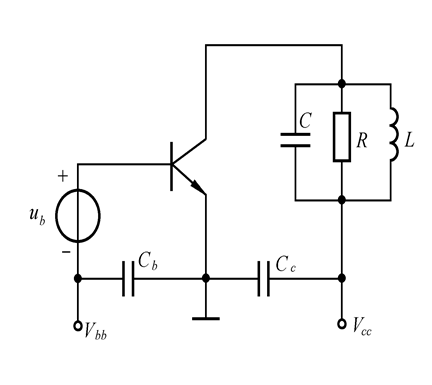
\includegraphics[width=1.8in]{fig/fig_rf_power_amp.png}
  \caption{RF Power Amplifier Load is resonant circuit}\label{fig_rf_power_amp}
\end{figure}

\subsubsection{Signal Generation}

\paragraph{LC oscillator} An Oscillator is basically an Amplifier  with ``Positive Feedback'', LC Oscillators are commonly used in radio-frequency circuits because of their good \emph{phase noise characteristics} and their \emph{ease of implementation}.

$$f=\frac{1}{2\pi \sqrt{LC}}$$

\begin{figure}
  \centering
  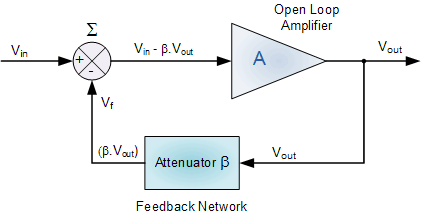
\includegraphics[width=2.0in]{fig/osc35.png}
  \caption{Block diagram of a feedback linear oscillator}\label{osc_diag}
\end{figure}

\subsubsection{Signal Modulation}

\paragraph{AM} The amplitude of the \emph{carrier wave} is varied in proportion to the waveform being transmitted. Set $c(t)=A\cdot sin(2\pi f_c t)$ as a carrier wave, and $m(t) = M \cdot cos(2 \pi f_m t + \Phi)$ is the modulation waveform. The amplitude modulated signal is:

\begin{align*}
  y(t) &= [ 1+ m(t)] \cdot c(t) \\
       &= A \cdot [ 1 + M ] \cdot cos(2 \pi f_m t + \Phi ) \cdot sin(2 \pi f_c t )
\end{align*}

\subparagraph{Envelope Detector} An envelope detector can be used to demodulate a previously modulated signal by removing all high frequency components of the signal, the corresponding circuit is shown in figure \ref{fig_rectified_voltagemeter}.

\paragraph{FM} Frequency Modulation (FM) is the encoding of information in a carrier wave by varying the instantaneous frequency of the wave. The frequency modulated signal is
$$u_{FM}(t)=Ucos[\omega_c t + k_f \int_{0}^{t} u_\Omega (t) dt]$$

\subparagraph{Direct Modulation} Direct FM modulation can be achieved by directly feeding the message into the input of a VCO.

\subparagraph{Ratio Detector} The ratio detector is not affected by amplitude variations on the FM wave. The output of the detector adjusts itself automatically to the average amplitude of the input signal.

The process of a ratio detector is:

$$FM\xrightarrow[\text{phase shift network}]{\text{frequency sensitive}}FM-PM\xrightarrow[]{\text{FM-PM + FM}}FM-AM\xrightarrow[\text{detector}]{\text{envelope}}u_\Omega(t)$$

\begin{figure}
  \centering
  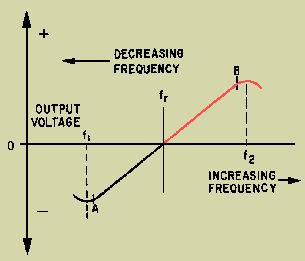
\includegraphics[width=2.5in]{fig/0260.png}
  \caption{Discriminator response curve}\label{fig_discriminator_respc}
\end{figure}

It uses a double-tuned RF transformer to convert frequency variations in the received FM signal to amplitude variations(\textbf{AM-FM}). A typical discriminator response curve is shown in figure \ref{fig_discriminator_respc}.

\subparagraph{Modulation Index} The value of the modulation index indicates by how much the modulated variable varies around its unmodulated level. It relates to variations in the carrier frequency:

$$h = \frac{\Delta{}f}{f_m} = \frac{f_\Delta |x_m(t)|}{f_m} $$

where $f_m$ is the highest frequency component present in the modulating signal $x_m(t)$ and $\Delta{}f$ is the peak frequency-deviation.

\paragraph{Mixer} RF mixing enables signals to be converted to different frequencies and thereby allowing the signals to be processed more effectively.

\begin{figure}
  \centering
  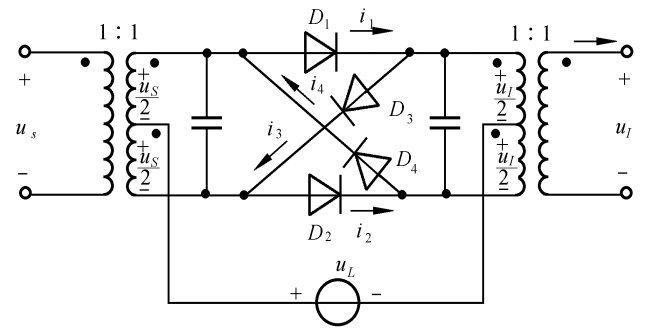
\includegraphics[width=3.2in]{fig/double-balanced-mixer.png}
  \caption{Basic double balanced diode mixer circuit}\label{fig_mixer}
\end{figure}

\begin{align*}
  i'  &= i_1-i_2=g_dk(\omega_Lt)(u_S-u_I) \\
  i'' &= i_3-i_4=g_dk(\omega_Lt-\pi)(u_S+u_I) \\
  i_I &= g_dU_{sm}\cos\omega_st-\frac{2}{\pi}g_dU_{Im}\cos\omega_st
\end{align*}

\subsubsection{Feedback Control}
\paragraph{PLL} A phase-locked loop (PLL) is a control system that generates an output signal whose phase is related to the phase of an input signal.
\begin{figure}
  \centering
  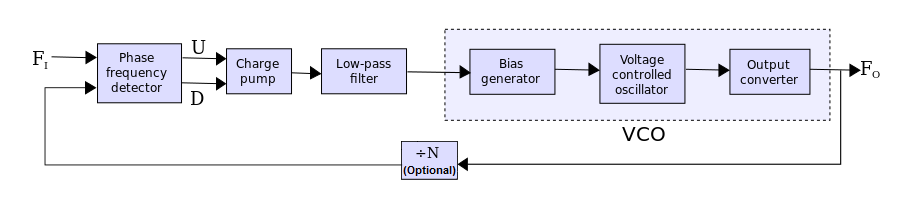
\includegraphics[width=4.5in]{fig/PLL_generic_inline_optional_N.png}
  \caption{Block diagram of a phase-locked loop}\label{fig_PLL}
\end{figure}

\paragraph{DDS} Direct Digital Synthesizer (DDS) is a type of frequency synthesizer used for creating arbitrary waveforms from a single, fixed-frequency reference clock.

\begin{figure}
  \centering
  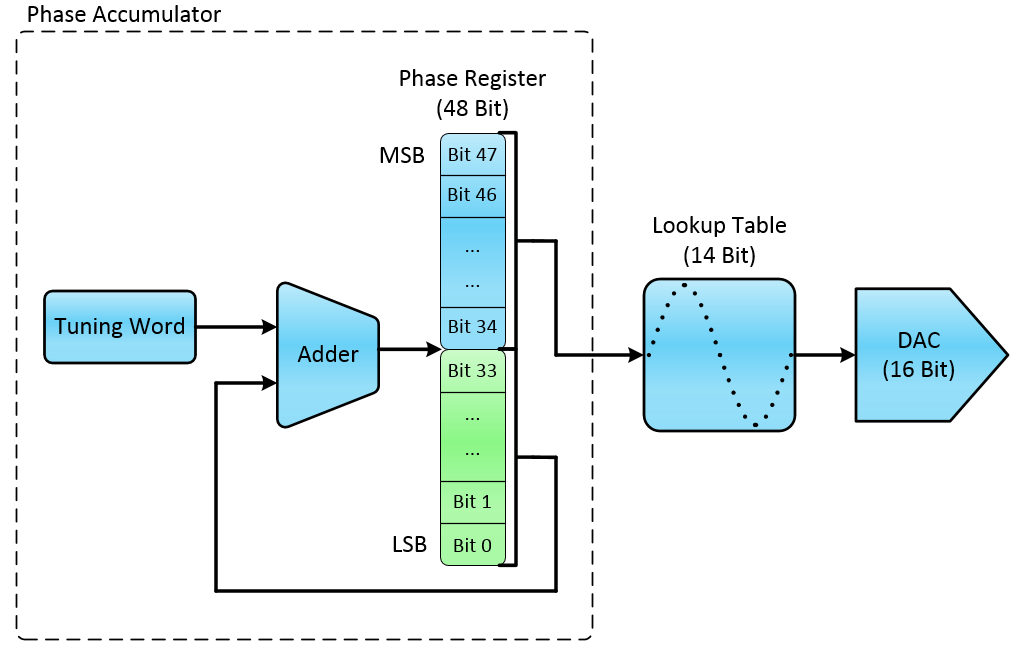
\includegraphics[width=3.5in]{fig/Fig_2_DDS_Block_Diagram.png}
  \caption{Hardware Block Diagram for the DDS Architecture}\label{fig_DDS}
\end{figure}

\subparagraph{Lookup Table}

The output of the phase register only looks like a digital ramp as the memory address increases over time, which is changing at the rate specified by the \emph{tuning word}. 
\section{Mechanik}
\subsection{Descriptive Geometry and Mechanical Drawing I}
One of the best ways to communicate one's ideas is through some form of picture or drawing. In this course, I've learnt about the basis of mechanical drawing, including: Use of Drawing Instruments, Orthographic Drawing, Sectioning, Dimensioning and ``Assembly'' Drawings.
\paragraph{Sectioning} There are many times when the interior details of an object cannot be seen from the outside. We can get around this by pretending to cut the object on a plane and showing the "sectional view".
\begin{figure}
  \centering
  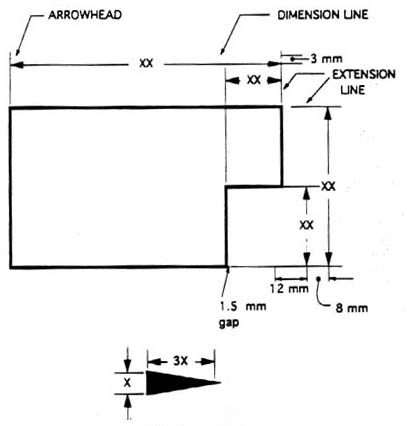
\includegraphics[width=2.4in]{fig/fig_dimensioned.jpg}
  \caption{Dimensioned Drawing}\label{fig_Dimensioned_Drawing}
\end{figure}

\begin{figure}
  \centering
  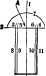
\includegraphics[width=0.3in]{fig/drawing-0111-2.jpg}
  \caption{bolt}\label{fig_bolt}
\end{figure}

\begin{figure}
  \centering
  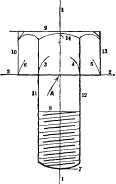
\includegraphics[width=0.4in]{fig/drawing-0112-1.jpg}
  \caption{bolt with a hexagon head}\label{fig_bolt1}
\end{figure}

\begin{figure}
  \centering
  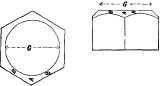
\includegraphics[width=1.1in]{fig/drawing-0121-1.jpg}
  \caption{nut}\label{fig_nut}
\end{figure}

\begin{figure}
  \centering
  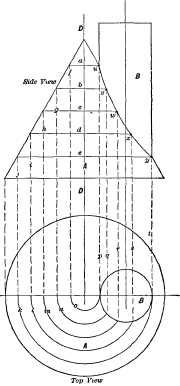
\includegraphics[width=0.9in]{fig/drawing-0189-1.jpg}
  \caption{a cylinder intersects a cone}\label{fig_projection}
\end{figure}

\subsection{Mechanics Base II}
This is a six-in-one course focus on mechanics design for non mechanics majors. The course talks about Planar Four-Bar Linkage, Cams, Statics, Mechanics of Materials, Shaft, Bearing, Gearing, as well as Tolerance and Fastener. I've learnt how to design a Axle or a gearbox, and how to choose bearings.

本课程主要讲述六个学科的主体内容,即理论力学、材料力学、机械原理、机械零件、仪器零件、公差,是非机类专业必修的一门主干课程。主要讲述机械中通用零、部件及常用机构的工作原理及设计方法。主要内容有静力学(Statics)、材料力学(mechanics of materials)、平面四连杆机构(Planar four-bar linkage)、齿轮传动(gearing)、凸轮(cams)、螺旋传动、轴(Axle)、轴承(bearing)、导轨(slide guide)、弹性元件(elastic element)、联接(Fastener)、公差(tolerance)。

\subsubsection{Planar four-bar linkage}
The synthesis, or design, of four bar mechanisms is important when aiming to produce a desired output motion for a specific input motion.

\paragraph{Grashof condition} If the sum of the shortest and longest link of a planar quadrilateral linkage is less than or equal to the sum of the remaining two links, then the shortest link (crank) can rotate fully with respect to a neighboring link.
\begin{figure}
  \centering
  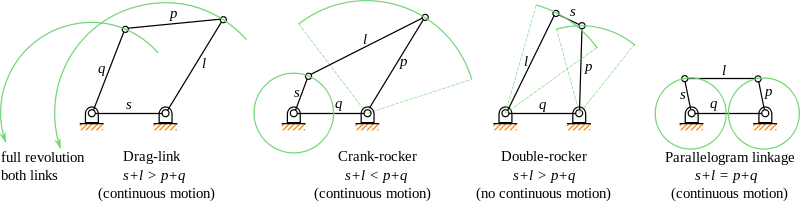
\includegraphics[width=4.5in]{fig/800px-Linkage_four_bar.svg.png}
  \caption{Types of four-bar linkages, s = shortest link, l = longest link. In the caption of the first figure, one must read s + l < p + q.}\label{fig_four_bar_linkage}
\end{figure}

\subsubsection{Cam}
A Cam is a machine component that either rotates or moves back and forth (reciprocates) to create a prescribed motion in a contacting element known as a follower. Cam systems can replace relatively complicated linkages in achieving desirable motion cycles.

\subsubsection{Mechanics of Materials}
Mechanics of Materials is a subject which deals with the behavior of solid objects subject to stresses and strains. Shear and bending moment diagrams are analytical tools used in conjunction with structural analysis to help perform structural design by determining the value of shear force and bending moment at a given point of a structural element such as a beam.

\begin{figure}
  \centering
  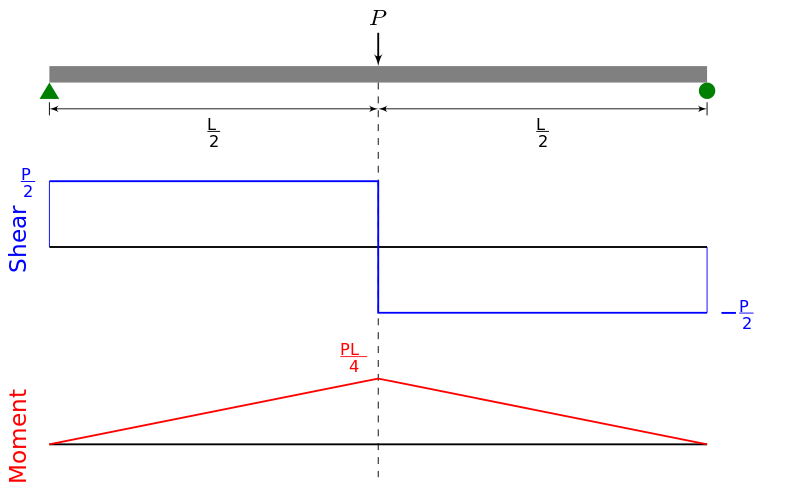
\includegraphics[width=4.2in]{fig/Shear_Moment_Diagram.svg.png}
  \caption{Shear and moment diagram for a simply supported beam with a concentrated load at mid-span.}\label{fig_Shear_Moment_Diagram}
\end{figure}

\subsubsection{Bearing}
The traditional method to estimate the life of the rolling-element bearings uses the basic life equation:
$$L_{10} = (C/P)^p \mbox{    }10^6 r$$

Where:

$L_{10}$ is the `basic life' (usually quoted in millions of revolutions) for a reliability of 90\%, i.e. no more than 10\% of bearings are expected to have failed

$C$ is the dynamic load rating of the bearing, quoted by the manufacturer

$P$ is the equivalent dynamic load applied to the bearing

$p$ is a constant: 3 for ball bearings, and 3.33 for roller bearings

\subsubsection{Gear}
A gear is a rotating machine part having cut teeth, which mesh with another toothed part in order to transmit torque.

Two or more gears working in tandem are called a transmission and can produce a mechanical advantage trough a gear ratio and thus may be considered a simple machine.

\paragraph{Gear Selection}
\begin{itemize}
  \item Pitch
  \item Face width
  \item Material
  \item Pressure angle
  \item \# of teeth
\end{itemize}

\paragraph{Worm gear} Worm-and-gear sets are a simple and compact way to achieve a high torque, low speed gear ratio.

\paragraph{Planetary Gear Trains}
\begin{figure}
  \centering
  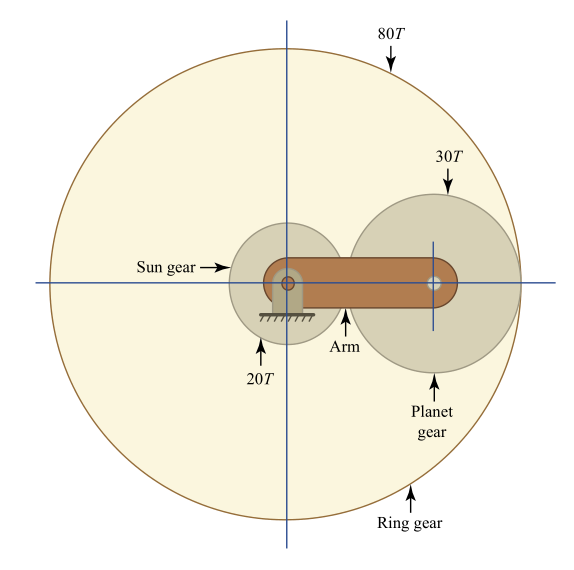
\includegraphics[width=3.2in]{fig/fig_planetary.png}
  \caption{Planetary Gear Trains}\label{fig_planetary}
\end{figure}

$$\mbox{Gear ratio   } e=\frac{n_L-n_A}{n_F-n_A}$$
where $n_L$: speed of last gear,

$n_A$: speed of arm,

$n_F$: speed of first gear(the sun)

\subsubsection{Coupling}
Couplings with parallel side keys are suitable for transfer of torsional moments, mostly in the same direction of rotation. Couplings with straight-sided splines are suitable for transfer of great, cyclical and shock torsional moments.

\begin{figure}
  \centering
  
\includegraphics[width=1in]{fig/220px-Spur_Gear_12mm,_18t.svg.png}
  \caption{Spur Gear}\label{fig_spur}
\end{figure}
\begin{figure}
  \centering
  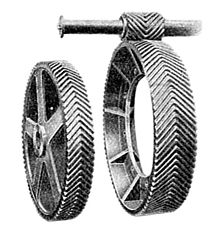
\includegraphics[width=1in]{fig/220px-Herringbone_gears_(Bentley,_Sketches_of_Engine_and_Machine_Details).jpg}
  \caption{Double helical}\label{fig_helical}
\end{figure}
\begin{figure}
  \centering
  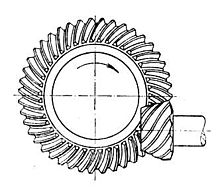
\includegraphics[width=1in]{fig/File-Sprocket35b.jpg}
  \caption{Bevel Gear}\label{fig_bevel}
\end{figure}
\begin{figure}
  \centering
  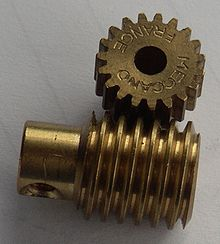
\includegraphics[width=1in]{fig/220px-Worm_Gear_and_Pinion.jpg}
  \caption{Worm gear}\label{fig_worm}
\end{figure}


\subsection{Sensing Technology and Its Applications}
In this course, I've got the basic knowledge of sensors, and several types of sensors, including resistance transducers, capacitor transducers, and inductance transducers, thermocouple, and optical sensors.

Sensors detect various physical parameters, and they are for gathering information, and for controlling systems.

A transducer is composed of Sensing element and Signal conditioning element.

\paragraph{Specifications}
\begin{itemize}
  \item Accuracy
  \item Linearity
  \item Sensitivity
  \item Repeatability
  \item Response time
\end{itemize}

\subsubsection{Resistance Transducers}
\paragraph{Strain Gauges} Resistance Strain Gauges are transducers which exhibit a change in electrical resistance in response to mechanical strain.

\paragraph{Resistance Temperature Detector (RTD)}
The RTD element is made from a pure material, typically platinum, nickel or copper. RTDs in industrial applications are rarely used above $660^{\circ}C$.

For Platinum RTD: $R_t=R_0[1+At+Bt^2]$
\subparagraph{Advantage}
\begin{itemize}
  \item High accuracy
  \item Low drift
  \item Wide operating range
  \item Suitability for precision applications
\end{itemize}

\subsubsection{Thermocouples}
All electrically conducting materials produce a thermal e. m. f., this is called the \emph{Seebeck effect}. When two different materials are connected to create a $T^\circ C$, a voltage is generated.

Advantages:
\begin{itemize}
  \item Capable of being used to directly measure temperatures up to $2600^{\circ}C$.
\end{itemize}

Disadvantages:
\begin{itemize}
  \item requires two temperatures be measured
  \item not linear
\end{itemize}

\subsubsection{Capacitor Transducers}
The capacitive transducer is used extensively for the measurement of displacement, pressure etc. The capacitive transducer or sensor is nothing but the capacitor with variable capacitance.
$$C=\frac{\varepsilon S}{d}=C_0+\Delta C = \frac{\varepsilon S}{d-\Delta d}=\frac{C_0}{1-\frac{\Delta d}{d}}$$

\begin{figure}
  \centering
  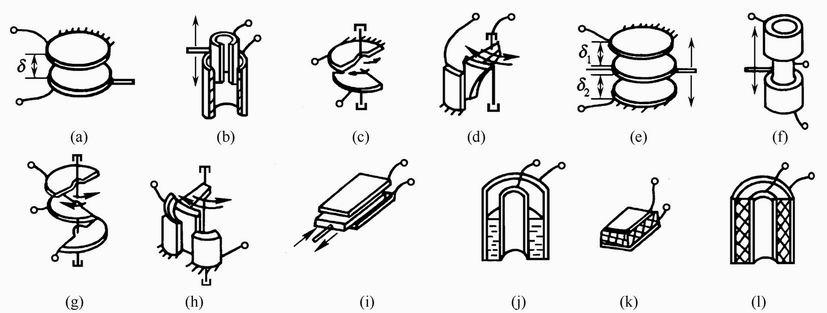
\includegraphics[width=4.2in]{fig/fig_capacitor.jpg}
  \caption{Capacitor Transducers}\label{fig_capacitor}
\end{figure}

Depending on the parameter that changes for the capacitive transducers, they are of three types as mentioned below.
\begin{itemize}
  \item Changing Dielectric Constant type of Capacitive Transducers
  \item Changing Area of the Plates of Capacitive Transducers
  \item Changing Distance between the Plates of Capacitive Transducers
\end{itemize}

Advantages:
\begin{itemize}
  \item It produces an accurate frequency response to both static and dynamic measurements.
\end{itemize}

Disadvantages:
\begin{itemize}
  \item An increase or decrease in temperature to a high level will change the accuracy of the device.
  \item As the lead is lengthy it can cause errors or distortion in signals.
\end{itemize}

\subsubsection{Inductive Transducer}
This type of transducer is used for finding the linear displacement in terms of voltage or other digital parameters.

Inductive transducers can be classified as follows:
\begin{enumerate}
  \item Variable self inductance: single coil, two coil
  \item Variable mutual inductance: simple two, three coil
  \item Variable reluctance: moving iron, moving coil, moving magnet
\end{enumerate}

\begin{figure}
  \centering
  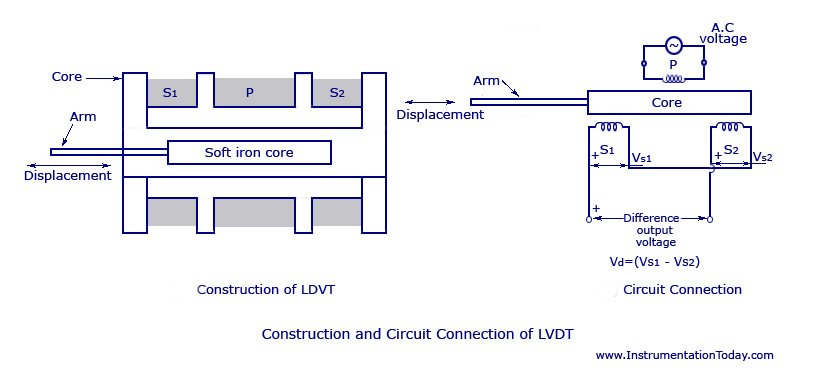
\includegraphics[width=4.2in]{fig/LVDT-Construction.jpg}
  \caption{Linear Voltage Differential Transformer (LVDT) Construction}\label{fig_LVDT}
\end{figure}

LVDT Advantages:
\begin{itemize}
  \item Maintains a linear relationship between the voltage difference output and displacement from each position of the core for a displacement of about 4 millimeter.
  \item Produces low hysteresis and thus has easy repeatability.
\end{itemize}

LVDT Disadvantages:
\begin{itemize}
  \item The whole circuit is to be shielded as the accuracy can be affetced by external magnetic field.
  \item A demodulator will be needed to obtain a d.c output.
  \item The efficiency of the device is easily affected by temperature.
\end{itemize}

\begin{figure}
  \centering
  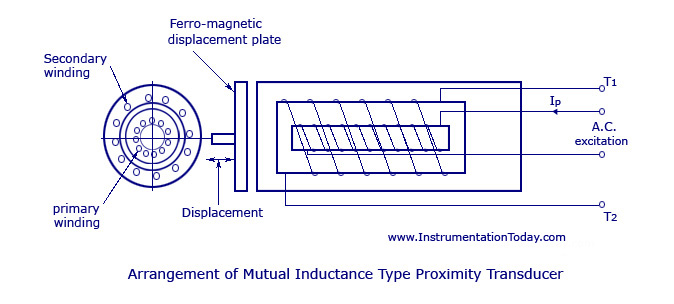
\includegraphics[width=4.2in]{fig/Proximity-Inductive-Transduccers.jpg}
  \caption{Proximity Inductive Transducers}\label{fig_proximity_inductive}
\end{figure}


\begin{figure}
  \centering
  \includegraphics[width=3.5in]{fig/Image22.png}
  \caption{Simple self inductance arrangement}\label{fig_inductance}
\end{figure}

\paragraph{Magnetic Transducers}
The Hall effect is the production of a voltage difference (the Hall voltage) across an electrical conductor, transverse to an electric current in the conductor and a magnetic field perpendicular to the current.

$F_L=evB$, $F_E=-eE_H=-eU_H/b$,

when $F_L+F_E=0$, $vB=U_H/b$

as $j=-nev$, $I=jbd=-nevbd$, and $v=-I/(nebd)$.

Thus:
$$U_H=-\frac{BI}{ned}=R_H\frac{IB}{d}=k_HIB$$
where $R_H$ is Hall coefficient.

Advantages:
\begin{itemize}
  \item not affected by ambient conditions, such as dust, humidity, and vibrations
  \item do not have contact with neighboring mechanical parts
  \item A high speed operation is possible.
\end{itemize}

Disadvantages:
\begin{itemize}
  \item Temperature affects the electrical resistance of the element and the mobility of majority carriers and also the sensitivity of Hall Effect sensors.
  \item An offset voltage occurs when there are physical inaccuracies and material non-uniformities.
\end{itemize}

\begin{figure}
  \centering
  \includegraphics[width=2.5in]{fig/fig_Hall.png}
  \caption{Hall Effect}\label{fig_hall}
\end{figure}

\subsubsection{Optic Transducers}
\begin{itemize}
  \item Photoemissive (Photodiodes/Phototransistors)
  \item Photoconductive (Photoresistors)
  \item CCD (Charge-coupled device)
\end{itemize}

\subsection{Project Design in Fundamentals of Mechanics}
\subsection{Engineering Training (Metalworking Practice)}
\subsection{Engineering Training (Electronic Processing Practice)}
In the practice, I've build up a radio by myself. The first thing to learn is Schweissen, then printed circuit board. After that, I placed the discrete components on the board, and began to schweissen. Finally, I managed to hear sound from the radio. 
\section{Computer}
\subsection{C Programming Language I}
This is a basic course about computer programming, the teacher lectures with C language, the most widely used in the area of engineering.

\subsection{Principles and Applications of MCU}
This course introduces the use of 8051 MCU. First assembly language is introduced, then the concept of timer, interrupt vector table, GPIO, and then the peripheral devices(LCD, keypad, etc...) A large part of the course is experiment, we make design and implementation on the physical chips, for example matrix keyboard.

\subsection{Project Design in Principles and Applications of MCU}
This is a practical course that requires the student team up and write a programme to control a robotic toy car. One of the three function must be implemented: tracing, speed measurement, and collision avoidance.

I've chosen the tracing one. We've given two linear CCD. On the playground there was a circle marked by black line. CCD returns high voltage when it senses light, and low voltage when dark, which indicates the deflection from the trace.

\subsection{Fundamentals of Engineering Software}
This course introduces the basis of computer software, including:
\begin{itemize}
  \item Network
  \item Operating System
  \item Data Structure
  \item Data Base
  \item Basis of Software Engineering
\end{itemize}

\paragraph{Network}
网络拓扑结构;ISO模型七层体系结构, 每层的功能;ISO模型与TCP/IP模型对应关系及差异;

\paragraph{Operating System}
固定分区分配;可变分区分配;分页、分段和段页存储管理;进程管理过程;设备管理的原理;

\paragraph{Data Base}
数据库相关概念;E-R图;范式;基本 SQL语言(查询);
\section{Pflichfach}
\subsection{Introduction of Automation Test and Opto-electrical Instrument}
This is a Fachkurs in the first semester, a introductory course. The teacher talks about what is measurement, and measurement that applied in different areas. The main part of the course introduces the graduate schools in our university.

\subsection{Error Theory and Digital Processing}
This course is consist of three parts: error theory, data processing, and uncertainty.
\paragraph{Error} Measurement error($e$) is the difference between a measured value($\hat{x}$) of quantity and its true value($X$). There are two types of measurement error: systematic errors and random errors.

$$e=|\hat{x}-X|$$

If parament $Y$ is acquired by indirect measurement

$$Y=a_1X_1+\dots+a_nX_n$$

then the measurement error of $Y$ is

$$\delta Y=\frac{\partial Y}{\partial X_1}\delta X_1 + \dots + \frac{\partial Y}{\partial X_n}\delta X_n$$

\paragraph{Linear Least Squares} It often happens that $A\mathbf{x}=\mathbf{b}$ has no solution. The usual reason is: too many equations. And this happens in measurement. We can get as much as measurement value as we want, and finally we want a better evaluation from the data we got. Assume we got a evaluation $\mathbf{x}$, then the evaluation error is $e=\mathbf{b} - A \mathbf{x}$. The smaller the error, the better the evaluation. And here comes the least squares.

\subparagraph{Error Equations}
set $v_i$ is the error with measurement value $l_i$, the true value is $f_i(x_1, x_2, \dots, x_t)$, its evaluation $y_i = a_{i1}x_1+a_{i2}x_2+\dots a_{it}x_t$. The error equations is:

\begin{equation*}
\left.
  \begin{array}{lr}
    v_1 = l_1 - y_1, &  \\
    v_2 = l_2 - y_2, & \\
    \dots \\
    v_n = l_n - y_n
  \end{array}
\right\}
\end{equation*}

In matrix form:
\begin{equation*}
  \begin{bmatrix}
    v_1 \\
    v_2 \\
    \vdots \\
    v_n
  \end{bmatrix}
  =
  \begin{bmatrix}
    l_1 \\
    l_2 \\
    \vdots \\
    l_n
  \end{bmatrix}
  -
  \begin{bmatrix}
    a_{11} & a_{12} & \ldots & a_{1t} \\
    a_{21} & a_{22} & \ldots & a_{2t} \\
    \vdots & \vdots & \ddots & \vdots \\
    a_{n1} & a_{n2} & \ldots & a_{nt}
  \end{bmatrix}
  \begin{bmatrix}
    x_1 \\
    x_2 \\
    \vdots \\
    x_t
  \end{bmatrix}
\end{equation*}
which is
\begin{equation} \label{equ_error}
V=L-A\hat{X}
\end{equation}

The object is to minimize the error:
\begin{equation} \label{equ_squ_error}
V^TV=0
\end{equation}

Differentiating equation \ref{equ_squ_error} with respect to x, we get:
$$\textbf{min }A^TV=0$$

Substitute $V$ with equation \ref{equ_error}, we get:
\begin{equation*}\label{equ_lsq}
  (A^TA)\hat{X}=A^TL
\end{equation*}

Thus the optimal evaluation is:
\begin{equation*}
  \hat{X}=(A^TA)^{-1}A^TL
\end{equation*}

\subparagraph{Beispiel}
对三段刻线间距的各种组合量进行了测量,得如下测量数据(单位mm):
$l_1=x,l_2=x,\dots,l_6=x$
试给出这三段刻线间距的最小二乘估计量$x_1,x_2,x_3$及其标准不确定度。
\begin{equation*}
\left.
  \begin{array}{lr}
    v_1 = l_1 - x_1, &  \\
    v_2 = l_2 - x_2, & \\
    v_3 = l_3 - x_3, & \\
    v_4 = l_4 - (x_1+x_2), & \\
    v_5 = l_5 - (x_2+x_3), & \\
    v_6 = l_6 - (x_1+x_2+x_3)
  \end{array}
\right\}
\end{equation*}

\paragraph{Uncertainty} Diese grenzt einen Wertebereich ein, innerhalb dessen der wahre Wert der Messgröße mit einer anzugebenden Wahrscheinlichkeit liegt (üblich sind Bereiche für ungefähr 68 \% und ungefähr 95 \%).

\begin{itemize}
  \item Typ-A: Ermittlung aus der statistischen Analyse mehrerer statistisch unabhängiger Messwerte aus einer Messwiederholung.

  $$u=s=\sqrt{\frac{\sum_{i=1}^{n}v_i^2}{n-1}}$$

  \item Typ-B: Ermittlung ohne statistische Methoden.
\end{itemize}

The combined standard uncertainty of the output quantity $u_C(y)$ can be expressed via the standard uncertainties of the input quantities $u(x_i)$ as follows:
\begin{equation*}
  u_c(y)=\sqrt{[\frac{\partial Y}{\partial X_1} u(X_1)]^2+[\frac{\partial Y}{\partial X_2} u(X_2)]^2+\dots+[\frac{\partial Y}{\partial X_n}u(X_n)]^2}
\end{equation*}

Note that if $X_i$ is random error, then $u(X_i)$ should be multiplied by 1/N additionally.

\subparagraph{erweiterte Unsicherheit} Dieser Kennwert kennzeichnet einen Wertebereich, der den wahren Wert der Messgröße mit hoher Wahrscheinlichkeit enthält.

\subsection{Automatic Test System}
This course introduces several types of bus used in automated electronic test and measurement systems, including PC-DAQ, GPIB/IEEE-488, VXI, PXI, and LXI. The kernel of an ATS lies in Bus interface and Software.

\paragraph{ATS} An ATS is consist of a number of instruments and computer. It can accomplish a certain amount of testing task according to the instructions. The main components of an ATS is:

\begin{enumerate}
  \item instrument controller(typically an PC)
  \item instruction-driven instruments
  \item standard testing bus
  \item software and develop environments
\end{enumerate}

\paragraph{PC-DAQ} \emph{Data acquisition} is the process of sampling signals from the real world and converting the resulting samples into digital numeric values that can be manipulated by a computer.

\paragraph{IEEE-488} IEEE-488 is an 8-bit, electrically parallel bus, with 3 line for handshake(DAV/Data Valid, NRFD/Not Ready for Data, and NDAC/Data Not Accepted). Five lines are used for addressing, and the bus supports up to 31 possible devices, with the cable length of up to 20 metres. The devices are attributed with ``listener'', ``controller'', and ``talker''.

\subparagraph{SCPI} While IEEE-488.1 defines the hardware interface, the software standard still remains blank. And IEEE-488.2 comes with a set of software protocol. And SCPI was introduced as an industry standard, with a set of general commands that each type of devices must obey, which improves software portability.

\paragraph{VXI} VXI is the VMEbus eXtensions for Instrumentation. VXI was introduces as the increasing demand for data rate in testing area. It has more precise timing and synchronization, which improve measurement capability.

\subparagraph{Commander/Servant Hierarchies} The VXIbus defines a Commander/Servant communication protocol so you can construct hierarchical systems using conceptual layers of VXI devices. This structure is like an inverted tree.

All devices has a configuration registers, and the system can identify each VXI device(type, model and manufacturer, address space, and memory requirements). In addition, VXI also defines Message-Based devices, which are required to have communication registers using Word Serial Protocol that is very similar to IEEE 488 protocol.

\subparagraph{VISA} One of the most notable benefits of VISA(\emph{Virtual Instrument Software Architecture}) is its ability to significantly reduce the time and effort involved in programming different I/O interfaces. Instead of using a different API devoted to each interface bus, you can use the VISA API regardless of whether your system is controlled by GPIB, VXI, or a GPIB-VXI. VISA is maintained by VXIplug\&play alliance(VPP).

\subparagraph{IVI} While VISA provides an abstraction of I/O interface(GPIB, VXI, etc), the IVI(Interchangeable Virtual Instrumentation) aims to provide a standard for instrument drivers.

\paragraph{PXI} PXI is based on CompactPCI, and it offers all of the benefits of the PCI architecture including performance, industry adoption.

PXI adds a rugged CompactPCI mechanical form-factor, an industry consortium that defines hardware, electrical, software, power and cooling requirements. Then PXI adds integrated timing and synchronization that is used to route synchronization clocks, and triggers internally.

Most PXI instrument modules are register-based products.

\paragraph{LXI} The LXI Standard defines the communication protocols for instrumentation and data acquisition systems using Ethernet. The LXI Standard has three major elements:
\begin{enumerate}
  \item A standardized LAN interface that provides a framework for web based interfacing and programmatic control.(Type C)
  \item A trigger facility based on the IEEE 1588 Precision Timing Protocol that enables modules to have a sense of time.(Type B)
  \item A physical wired trigger system that tightly synchronizes the operation of multiple LXI instruments.(Type A)
\end{enumerate}

\subsection{Principles of Electronic Measurement}
This course focuses on the fundamentals and structure of electronic instrument. Time/frequency measurement, voltage measurement, the structure of oscilloscope, and frequency spectrum analyzer are covered. Among the items above, time/frequency measurement is the most significant technique, because all the rest technique directly or indirectly involved timing.

\subsubsection{Measuring Time/Frequency}

Time/Frequency measurement has the highest accuracy among others, and time is one of the most basic physical parameters. By definition, period and frequency has the following relationship:
$$f=\frac{1}{T}$$
\paragraph{Frequency} The input signal is initially conditioned to a form that is compatible with the internal circuitry of the counter. The conditioned signal appearing at the door of the main gate is a pulse train where each pulse corresponds to one cycle or event of the input signal. With the main gate open, pulses are allowed to pass through and get totalized by the counting register. The time between the opening to the closing of the main gate or gate time is controlled by the Time Base.

\begin{figure}
  \centering
  \includegraphics[width=4.5in]{fig/freq_counter.png}
  \caption{Basic block diagram of the conventional counter in its frequency mode of measurement}\label{fig_freq_counter}
\end{figure}

In a specified period $T$, the counter has its value of $N$, then by definition of the frequency, we get

$$f=\frac{N}{T}$$

\paragraph{Time} If we switch the port where frequency signal and time base signal are fed, then the frequency counter can be used for time measurement. By definition:

$$T=\frac{N}{f}$$
where $f$ is the frequency of time base signal.

\subsubsection{Measuring Voltage}

Voltage measurement is more important than other parameters, because others, such as current, power, temperature, pressure, can be converted to voltage.
For an alternating current, it is rectified and measured for RMS value by its \emph{average value} or \emph{peak value}. And the voltage meter presume that the signal is a sinusoidal signal. While peak envelope voltage meter has wider broadband(\SI{1000}{\mega\hertz}), average voltage has better sensitivity.

\begin{itemize}
  \item by converting to direct current

  Peak envelope value, or average value, or root-mean-square value can be converted to direct current.

  \item by calculating with mathematical calculation

  the analog voltage can be converted to digital signal by AD converter, which is easier to couple with.
\end{itemize}

\paragraph{Why RMS?} The purpose of RMS value is to \textbf{simplify power calculations} by providing equivalent DC voltage that would develop the same average power in resistive load.

\paragraph{Crest Factor} crest factor = |peak value| / rms value

\begin{figure}
  \centering
  \includegraphics[width=3.0in]{fig/fig_envelop_detector.png}
  \caption{Envelop Detector}\label{fig_envelop_detector}
\end{figure}

The crest factor for a sinusoidal current waveform is 1.414.

\paragraph{Form Factor} form factor = rms value / |average value|

The form factor for a sinusoidal current waveform is 0.9.

\begin{figure}
  \centering
  \includegraphics[width=2.5in]{fig/fig_rectified_voltmeter.png}
  \caption{Half Wave Rectifier Circuit for Average value Voltagemeter}\label{fig_rectified_voltagemeter}
\end{figure}

As shown in figure \ref{fig_rectified_voltagemeter}, the rectified voltage is then measured by a gauge.

\subsubsection{Structure of Oscilloscope}
The cathode-ray oscilloscope (C.R.O.) consists of the following components:
\begin{enumerate}
  \item Electron Gun
  \item Deflection System
  \item Display Screen
\end{enumerate}

\begin{figure}
  \centering
  \includegraphics[width=4.5in]{fig/fig_cro.png}
  \caption{Structure Of Cathode Ray Oscilloscope}\label{fig_crc}
\end{figure}

The electron gun generates electron beam, and deflected by the deflection system controlled by X input(horizonal) and Y input(vertical).

Y input is fed by signal to be measured, it may be amplified/attenuated, delayed in the Y channel. The structure of X channel is far more complicate than Y channel. The X channel should generate a signal that is proportional to time(sweeping), when new signal comes at Y channel(trigger).

\paragraph{Pulse generator} The trigger in X channel should generate a pulse to start sweeping circuit when the Y input reaches a certain voltage level(trigger voltage). A pulse may be trigged during sweep cycle, and it should be neglected.

\paragraph{Sweep generator} The sweep generator should produce one cycle of a sawtooth waveform, when it receives a pulse at its input. The period of a sawtooth waveform can be decomposed to two stage: trace stage and flyback stage, as shown in figure \ref{fig_X_channel}.

\begin{figure}
  \centering
  \includegraphics[width=4.2in]{fig/fig_X_channel.png}
  \caption{Sawtooth waveform in X channel}\label{fig_X_channel}
\end{figure}

\subsubsection{Structure of Frequency Spectrum Analyzer}

There are two ways to display the spectrum of a signal: either by acquiring the envelope or by FFT calculation.

The technical parameters of a frequency spectrum analyzer includes:
\begin{itemize}
  \item input range - the maximum range that the analyzer can measure
  \item span - the range that the analyzer can scan once in a time
  \item frequency resolution - determined by IF filter
  \item sweep time - the time required to perform a scan
  \item phase noise - reflects the short-term frequency stability
\end{itemize}

\paragraph{Superheterodyne Spectrum Analyzer}

\begin{figure}
  \centering
  \includegraphics[width=4.5in]{fig/fig_spe_anlyzer.png}
  \caption{Block diagram of a classic superheterodyne spectrum analyzer}\label{fig_spe_anlyzer}
\end{figure}

Figure \ref{fig_spe_anlyzer} is a simplified block diagram of a superheterodyne spectrum analyzer.

\textbf{Heterodyne} means to mix; that is, to translate frequency. And \textbf{super} refers to superaudio frequencies, or frequencies above the audio range.

The input signal passes through an attenuator, then through a low-pass filter to a mixer, and is mixed with a signal from local oscillator(LO). The low-pass filter here is to ease noise from higher frequency, as shown in figure \ref{fig_spectrum_analyser}: $f_L = f_X + f_{IF}$.

\begin{figure}
  \centering
  \includegraphics[width=3.5in]{fig/fig_spectrum_analyser.png}
  \caption{the process of spectrum translation}\label{fig_spectrum_analyser}
\end{figure}

It is essentially rectified by the envelope detector, filtered through the low-pass filter and displayed. A ramp generator creates the horizontal movement across the display from left to right. The ramp also tunes the LO so its frequency change is in proportion to the ramp voltage.

\begin{figure}
  \centering
  \includegraphics[width=4.2in]{fig/fig_phase_noise.png}
  \caption{Phase noise is displayed only when a signal is displayed far enough above the system noise floor}\label{fig_phase_noise}
\end{figure}

\paragraph{FFT Spectrum Analyzer} The FFT Spectrum Analyzer samples the filtered signal and converts into digital series, then FFT is conducted in microprocessor. It uses digital signal processing techniques to provide in depth waveform analysis with greater flexibility than other methods.

\subsection{Process Control Techniques and Systems}
The main topic of the course is process control system and corresponding control technique.

\subsubsection{Basic Terms}

\paragraph{Process} \emph{Process} refers to the methods of changing or refining raw material(mostly fluid) to create end products.

\paragraph{Process Variable} A \emph{process variable} is a condition that can change the manufacturing process in some way, such as pressure, flow, temperature, pH.

\paragraph{Process control} \emph{Process control} refers to the methods that are used to control process variables(temperature, humidity, etc) when manufacturing a product.

\paragraph{Setpoint} The \emph{setpoint} is a value for a process variable be expected to maintained.

\paragraph{Offset} \emph{Offset} is a sustained deviation from the setpoint.

\subsubsection{Control Loop Components}

There devices that implements the task of measurement, Komparation, and adjustment in the control loop:

\begin{itemize}
  \item sensor
  \item transducer

  A \emph{transducer} is a device that translates a mechanical signal into a electrical signal.

  \item converter

  A \emph{converter} is a device that converts one type of signal into another type of signal, for example \SIrange{4}{20}{\milli\ampere} current signal into another form of pressure signal.

  \item transmitter

  A \emph{transmitter} is a device that converts a signal from sensor/transducer into standard signal and transfers that signal to a monitor or a controller.

  \item indicator
  \item recorder
  \item controller

  A \emph{controller} reads signals from sensor, and output control signal to actuator.

  \item actuator

  An \emph{actuator} is a device that undertakes the task to change the process variables.
\end{itemize}

\subsubsection{Control Algorithms}

\paragraph{PID} The most commonly used control algorithm, P stands for proportional, I stands for integral, and D stands for differential.

\paragraph{Feed forward control} Feed forward control can ease the effect of any disturbance that can be measured.

\paragraph{Smith Predictor} The Smith predictor is a type of predictive controller for systems with \emph{pure time delay}. Subtracting the disturbance-free process variable from the actual process variable yields an \emph{estimate of the disturbances}. By adding this difference to the predicted process variable, Smith created a feedback variable that includes the disturbances, but not the deadtime.

\begin{figure}
  \centering
  \includegraphics[width=3.5in]{fig/Smith_control2.jpg}
  \caption{Block Diagram of Smith Predictor}\label{fig_smith}
\end{figure}

\subsection{Fundamentals Design of Intelligent Instruments}
This course covers the structure of an instrumentation from microprocessors, Sampling, Human-machine Interfaces, communication interfaces and software developments.

\subsubsection{Sampling}

\begin{figure}
  \centering
  \includegraphics[width=2.5in]{fig/sample_channel.png}
  \caption{Simultaneous Sampling Architecture}\label{fig_sample_channel}
\end{figure}

The structure of a sampling channel is as follows:

\begin{itemize}
  \item multiplexer
  \item sample\& hold circuit
  \item AD converter
\end{itemize}

\paragraph{Signal Conditioning} Input signal may be amplified by front-end amplifier. Front-End amplifiers are mainly used to improve the signal to noise ration at the receiver.

In order to get highest resolution from ADC, the input signal should be amplified in the full range of ADC. The amplifier should have high input impedance, high input bandwidth, high CMRR, low drift, low output noise, and low output impedance.

\begin{figure}
  \centering
  \includegraphics[width=2.5in]{fig/SHA_circuit.png}
  \caption{Sample \& Hold Circuit}\label{fig_SHA}
\end{figure}

\paragraph{AD converter} Three types of AD converter are most applied:

\begin{itemize}
  \item Successive approximation ADC

  low power consumption, high resolution and accuracy, and a small form factor

  \item Slope(integrating) ADC

  high accuracy, low speed, needs external components

  \item $\Sigma - \Delta$ ADC

  high resolution, no calibration needed, no external components

\end{itemize}

\begin{figure}
  \centering
  \includegraphics[width=4.5in]{fig/sigma_delta_ADC.png}
  \caption{Sigma-Delta ADC}\label{fig_sigma_delta_ADC}
\end{figure}


\begin{figure}
  \centering
  \includegraphics[width=2.5in]{fig/SA_ADC_block_diagram.png}
  \caption{SAR ADC}\label{fig_SAR_ADC}
\end{figure}


\paragraph{Error} Here is a list of errors in the sampling system:
\begin{itemize}
  \item sampling error

  According to Nyquist's theorem, if the signal has frequency of $f_s$, then the sampling system should be $2f_s$ or higher in order to reduce aliasing. So, for an N channel simultaneous sampling system, the minimum frequency required should be $2Nf_s$.

  \item analog circuit error

  Analog circuit error comes from sensor, amplifier, multiplexer, sample \& hold circuit.

  \item ADC error

  Temperature Drift
\end{itemize}

\subsubsection{Human-machine Interface}

Human-machine Interfaces include matrix keypad, LED segment display, and touch screen.

It is important to remove keypad jitter, either by hardware(capacitor) or by software(programmed delay).

\begin{figure}
  \centering
  \includegraphics[width=2.2in]{fig/4x3_KeypadLayout.png}
  \caption{4x3 Keypad Layout}\label{fig_keypad}
\end{figure}

If more command are expected than the number of keys on the keypad, then a state machine may be introduced.

\subsubsection{Reliable Software Development}

An instrument may perform self test upon initialization or during runtime, and the content of self test can include circuit, memory(RAM, ROM), bus, keypad, display, etc.

\paragraph{Common Mode Rejection} Common mode rejection may be achieved via following:

\begin{itemize}
  \item differential amplifier
  \item voltage transformer/optical coupling
  \item isolation amplifier
  \item floating ground
\end{itemize}

\subsection{Comprehensive Specialty Experiment}
This is the last course in the university. The students are asked to contact with his/her tutor for a topic to be investigated. My tutor asked me to do a research on the current development of ambient air pollution monitor system and write a review.

\subsubsection{Measurement Component}

\paragraph{Rotatory Encoder} The encoder consists of a light source (LED) and an array of photo-detectors, separated by a slotted disc known as a code wheel. The disc is mounted on the rotating motor shaft. Each time a slot passes between the LED and a detector, the detector receives a flash of light and generates an electrical pulse. 

\subsection{Production Practice}
This is a practical course. The course takes two week: one week in local and the other in Dalian. I paid a visit to several companies, such as Harbin Electric Machinery Company Limited and Dalian Locomotive and Rolling Stock Co., LTD. 
\section{Wahlpflichtfach}

\subsection{Introduction to photonics and optical sensor}
The main contents are the basically theory and the principle of the field of photonics. The course covers the laser, optical waveguide, optical fiber and optical sensor with the relation of the optical measurement.

\subsection{Reconfigurable Computing}

\subsection{DSP Principle and Applications}

This course introduces the basis of Digital Signal Processor. The type of DSP to be analyzed is TI TMS320LF2407A.

\paragraph{Comparation} The table \ref{tab_chip} shows the differences between DSP, MCU, and ARM.

\begin{table}
  \centering
  \caption{Comparation between DSP, MCU, and ARM}
  \label{tab_chip}
  \begin{tabular}{|c|c|}
    \hline
    % after \\: \hline or \cline{col1-col2} \cline{col3-col4} ...
    Chip & Feature \\
    \hline
    DSP & optimized for real time signal processing \\
    MCU & low price, easy to use \\
    ARM & able to run RTOS, rich function \\
    \hline
  \end{tabular}
\end{table}

\paragraph{Peripheral Interrupt} The interrupt in DSP is managed by PIE, which support up to 6 level interrupt sources. The priority of interrupts can be divided into two types: lower priority interrupts generates an INTn from PIRQ, and higher priority interrupts from INTn are send to CPU.

The following is the sequence to enable an interrupt:

\begin{enumerate}
  \item *EVAIMRA = 0x80;/* 使能T1周期中断 */
  \item *IMR=0x2;   /* 使能定时器中断(INT2) */
  \item asm(``clrc INTM'');
\end{enumerate}

\paragraph{Memory} TMS320LF2407A has three memory space, with each size of \SI{64}{\kibi\byte}:
\begin{itemize}
  \item I/O space
  \item data space
  \item program space
\end{itemize}

\subsection{Machine Vision and Application}

In this course I learnt about the basic concept of machine vision, the structure of a vision system, and the fundamental theory of digital image processing.

Machine Vision is not limited to visible light, and it can be extended to the image of sound, microwave, and infrared ray. This broadens the horizon of the human eye.

\paragraph{Structure} A vision system is consist of the following components:
\begin{itemize}
  \item light source
  \item camera
  \item CCD(charge coupled device)
  \item data acquisition card
  \item image processing software
\end{itemize}

\paragraph{Low Level Image Processing} The task for low-level image processing is to refine/enhance the image, by filter, edge detection, image enhancement, image transformation, etc. The purpose is to provide the refined image for further, higher level image processing.

\paragraph{High Level Image Processing} The high level image processing is to undertake the task that requires intelligence, such as pattern recognition, image classification, target tracing, etc.

\paragraph{Application} Machine Vision is applied in the manufacturing of electronic products: counting the pins of a chip. And robot also needs vision for guidance. Remote sensing needs machine vision for analytical purpose.

\subsection{Automatic Control Components and Equipment}

This course mainly introduces the basic principal theory of drive Servo Motor including DC, AC, Step motors. The measurement component: measuring motor, rotation transfer and light-electric code are also explained. The course purpose is to teach the students to design and analysis the common electrical control system independently.

\subsubsection{Motor}

A motor transfer electric power into mechanic power, and a generator im Gegenteil umwandelt mechanische Energie in elektrische Energie.

\paragraph{Construction}

A motor is consist of following components:
\begin{itemize}
  \item Rotor

  In an electric motor the moving part is the rotor which turns the shaft to deliver the mechanical power.

  \item Stator

  The stator is the stationary part of the motor's electromagnetic circuit and usually consists of either windings or permanent magnets.

  \item Air gap

  The distance between the rotor and stator is called the air gap. The air gap increases magnetizing current. For this purpose air gap should be minimum.

  \item Windings

  \item Commutator

  A commutator is a mechanism used to switch the direction of direct current for most DC motors.
\end{itemize}

\paragraph{DC Motor} The stator of a DC motor is mostly permanent magnetics. When the motor powers up, the current goes through rotor and creates an electromagnetic forces that drives the rotor to rotate. A DC motor needs a commutator to switch current direction.

\paragraph{AC Motor} AC motor ist mit Dreiphasenwechselstrom betrieben. The three phase altering current forms a rotierende Magnetfeld that drives the rotator to rotate.

AC motor is asynchronous to the Magnetfeld, which is cause by the nature that the motor is driven by magnetic force that besteht aus relative movement.

\paragraph{Step Motor} The stepper motor is known by its property to convert a train of input pulses (typically square wave pulses) into a precisely defined increment in the shaft position. \subsection{Introduction to the History of World Civilization}
This course introduced the main line of the history of world civilization. The main part includes: mesopotamia, ancient Greek and ancient China. Mesopotamia is a special place, many civilizations immigrates in, and some others die out. Two main parts are: Sumerian Civilization and Semitic civilization.

\subsection{Intellectual Property Law}
This course introduces the basis of intellectual property law. This right has no physical body, has time limit and monopoly, and has geometrical limitation. It includes patent copyright, trademarks, etc... 
\section{Nebenfach} 

\subsection{Study of Famous Figures in Contemporary and Modern China}
This course introduces some of the famous figures in the contemporary and modern China, for example Hu Shi(胡适).

\subsection{Electronic Controlling Technology for Automobile}
This course introduces structure of the control system in a automobile, including chassis control system and motor control system. And some technology applied to the chassis control, such as ABS, ESP are introduced.

\subsection{State-of-the-art of pattern}
This course introduces several algorithms in pattern recognition and its math in detail, including support vector machine(SVM), artificial neural network(ANN), Perceptron, Principal Component Analysis(PCA), Clustering, and Hidden Markov Model(HMM).

\subsection{Drive and Control of Integration Motor System}
This course gives the basic of electric motor, and technical introduction of vector control. Basically, a motor is composed of rotor, stator, air gap, windings, and motor control system.

\subsection{Infrared spectroscopy measuring instrument design}
This is a innovation course, mainly focus on experiment. By the end of the course, I have learnt the concept of infrared spectrum, how to calibrate spectroscopy. The sampled data are fitted with the true value via linear least square method.

\subsection{C Program of Control and Measurement System}
This course talks about system programming in control system. Devices includes: AD/DA and Step motor. The operating system is DOS, IDE is TuroboC. Experiments accounts for half the course, including DOS system programming and timer control, ADC and plotting, wave generation and DAC, step motor control.

\subsection{German as Second Foreign Language I}
This course introduces the very basis of German. In this course, I learnt about the spelling of German and its sentence structure, noun.

\subsection{German as Second Foreign Language II}
This course introduces Adjektiv, Dativ and Akkusativ, and in the end, the teacher introduced some basic concept of Genitiv.

\subsection{Piano Recital art entry}
This is a elective course. The teacher guided me how to play piano and left the most of time to practise. By the end of the course, I managed to play with both hands.

\subsection{An Introduction to Artificial Intelligence}
This course is about natural language processing. It introduces the N Gram module, Viterbi dynamic programming algorithm and Chinese word segmentation. By the end of the course, I managed to make a programming to perform Chinese word segmentation.

\subsection{Algorithm for Big Data}
This course introduces the concept of big data and its algorithms. The characteristics are volume, velocity, variety and value. Due to the limitation of memory, time, I/O and performance, algorithms are adapted to the enormous amount of data. One example is sub-linear time complexity algorithm. It features that only a small amount of data are stored in the memory, and data are feed into the programme(streaming).

\subsection{Introduction to photonics and optical sensor}
This course talks about Fibre Optical System Design. First the teacher talked about the steps for system design, and then the steps were applied to the fibre one. There are four steps involved:
\begin{enumerate}
  \item Evaluate requirements
  \item Make components selection
  \item Calculate power budget
  \item Calculate rise time budget
\end{enumerate}

\subsection{C/C++ senior advanced cases}
This is a experimental course, and the students group up to make a project from a list given by the teacher. I myself form a group. And by the end of the course, I managed to make a dictionary that supports simple regular expression(front, rear and wildcard).

\subsection{The Art of Piano Performance and Appreciation of Classical Music}

\subsection{Innovation Design of Communication \& Electronic systems} 

\end{document} 